%%%%%%%%%%%%%%%%%%%%%%%%%%%%%%%%%%%%%%%%%%%%%%%%%%%%%%%%%%%%%%%%%%%%%%%%%%%
%% This file is part of the book
%%
%% Algorithmic Graph Theory
%% http://code.google.com/p/graph-theory-algorithms-book/
%%
%% Copyright (C) 2010 David Joyner <wdjoyner@gmail.com>
%% Copyright (C) 2009, 2010 Minh Van Nguyen <nguyenminh2@gmail.com>
%%
%% See the file COPYING for copying conditions.
%%%%%%%%%%%%%%%%%%%%%%%%%%%%%%%%%%%%%%%%%%%%%%%%%%%%%%%%%%%%%%%%%%%%%%%%%%%

\chapter{Tree Data Structures}
\label{chap:tree_data_structures}

\begin{quote}
\includegraphics[scale=0.7]{image/tree-data-structures/tree.png} \\
\noindent
--- Randall Munroe\index{Munroe, Randall}, xkcd,
\url{http://xkcd.com/835/}
\end{quote}


%%%%%%%%%%%%%%%%%%%%%%%%%%%%%%%%%%%%%%%%%%%%%%%%%%%%%%%%%%%%%%%%%%%%%%%%%%%

\section{Priority queues}

A \emph{priority queue}\index{queue!priority} is essentially a queue
data structure with various accompanying rules regarding how to access
and manage elements of the queue. Recall from
section~\ref{subsec:graph_algorithms:breadth_first_search} that an
ordinary queue $Q$ has the following basic accompanying functions for
assessing and managing its elements:
%%
\begin{itemize}
\item $\dequeue(Q)$ --- Remove the front of $Q$.

\item $\enqueue(Q, e)$ --- Append the element $e$ to the end of $Q$.
\end{itemize}

If $Q$ is now a priority queue, each element is associated with a key
or priority $p \in X$ from a totally ordered\index{total order} set
$X$. A binary relation denoted by an infix operator, say ``$\leq$'',
is defined on all elements of $X$ such that the following properties
hold for all $a,b,c \in X$:
%%
\begin{itemize}
\item Totality: We have $a \leq b$ or $b \leq a$.

\item Antisymmetry: If $a \leq b$ and $b \leq a$, then $a = b$.

\item Transitivity: If $a \leq b$ and $b \leq c$, then $a \leq c$.
\end{itemize}
%%
If the above three properties hold for the relation ``$\leq$'', then we
say that ``$\leq$'' is a \emph{total order}\index{total order} on $X$
and that $X$ is a
\emph{totally ordered set}\index{set!totally ordered}. In all, if the
key of each element of $Q$ belongs to the same totally ordered
set $X$, we use the total order defined on $X$ to compare the keys of
the queue elements. For example, the set $\Z$ of integers is totally
ordered by the ``less than or equal to'' relation. If the key of each
$e \in Q$ is an element of $\Z$, we use the latter relation to compare
the keys of elements of $Q$. In the case of an ordinary queue, the
key of each queue element is its position index.

To extract from a priority\index{queue!priority} queue $Q$ an element
of lowest priority, we need to define the notion of smallest
priority or key. Let $p_i$ be the priority or key assigned to element
$e_i$ of $Q$. Then $p_{\min}$ is the lowest key if $p_{\min} \leq p$
for any element key $p$. The element with corresponding key
$p_{\min}$ is the minimum priority element. Based upon the notion of
key comparison, we define two operations on a priority queue:
%%
\begin{itemize}
\item $\insertElem(Q, e, p)$ --- Insert into $Q$ the element $e$ with
  key $p$.

\item $\extractMin(Q)$ --- Extract from $Q$ an element having the
  smallest priority.
\end{itemize}

An immediate application of priority queues is sorting a finite
sequence of items. Suppose $L$ is a finite list of $n > 0$ items on
which a total order is defined. Let $Q$ be an empty priority queue. In
the first phase of the priority queue sorting algorithm, we extract
each element $e \in L$ from $L$ and insert $e$ into $Q$ with key $e$
itself. In other words, each element $e$ is its own key. This first
phase of the sorting algorithm requires $n$ element extractions from
$L$ and $n$ element insertions into $Q$. The second phase of the
algorithm involves extracting elements from $Q$ via the $\extractMin$
operation. Queue elements are extracted via $\extractMin$ and inserted
back into $L$ in the order in which they are extracted from
$Q$. Algorithm~\ref{alg:tree_data_structures:priority_queue_sort}
presents pseudocode of our discussion. The runtime of
Algorithm~\ref{alg:tree_data_structures:priority_queue_sort} depends
on how the priority queue $Q$ is implemented.

\begin{algorithm}[!htbp]
%%%%%%%%%%%%%%%%%%%%%%%%%%%%%%%%%%%%%%%%%%%%%%%%%%%%%%%%%%%%%%%%%%%%%%%%%%%
%% This file is part of the book
%%
%% Algorithmic Graph Theory
%% http://code.google.com/p/graph-theory-algorithms-book/
%%
%% Copyright (C) 2009, 2010 Minh Van Nguyen <nguyenminh2@gmail.com>
%%
%% See the file COPYING for copying conditions.
%%%%%%%%%%%%%%%%%%%%%%%%%%%%%%%%%%%%%%%%%%%%%%%%%%%%%%%%%%%%%%%%%%%%%%%%%%%

\DontPrintSemicolon
\SetAlgoNoLine
%%
%% data section
\SetKwInOut{Input}{Input}
\SetKwInOut{Output}{Output}
%%
%% input/output
\Input{A finite list $L$ of $n > 0$ elements on which a total order is
  defined.}
\Output{The same list $L$ sorted by the total order relation defined
  on its elements.}
\BlankLine
%%
%% algorithm body
$Q \assign [\,]$\;
\For{$i \assign 1, 2, \dots, n$}{
  $e \assign \dequeue(L)$\;
  $\insertElem(Q, e, e)$\;
}
\For{$i \assign 1, 2, \dots, n$}{
  $e \assign \extractMin(Q)$\;
  $\enqueue(L, e)$\;
}

\caption{Sorting a sequence via priority queue.}
\label{alg:tree_data_structures:priority_queue_sort}
\end{algorithm}


%%%%%%%%%%%%%%%%%%%%%%%%%%%%%%%%%%%%%%%%%%%%%%%%%%%%%%%%%%%%%%%%%%%%%%%%%%%

\subsection{Sequence implementation}
\label{subsec:tree_data_structures:sequence_implementation}

A simple way to implement a priority queue is to maintain a sorted
sequence. Let $e_0, e_1, \dots, e_n$ be a sequence of $n + 1$ elements
with corresponding keys $k_0, k_1, \dots, k_n$ and suppose that the
$k_i$ all belong to the same totally ordered set $X$ having total
order $\leq$. Using the total order, we assume that the $k_i$ are
sorted as
\[
k_0 \leq k_1 \leq \cdots \leq k_n
\]
and $e_i \leq e_j$ if and only if $k_i \leq k_j$. Then we consider the
queue $Q = [e_0, e_1, \dots, e_n]$ as a priority queue in which the
head is always the minimum element and the tail is always the maximum
element. Extracting the minimum element is simply a dequeue operation
that can be accomplished in constant time $O(1)$. However, inserting a
new element into $Q$ takes linear time.

Let $e$ be an element with corresponding key $k \in X$. Inserting $e$
into $Q$ requires that we maintain elements of $Q$ sorted according to
the total order $\leq$. If $Q$ is empty, we simply enqueue $e$ into
$Q$. Suppose now that $Q$ is a nonempty priority queue. If
$k \leq k_0$, then $e$ becomes the new head of $Q$. If $k_n \leq k$,
then $e$ becomes the new tail of $Q$. Inserting a new head or tail
into $Q$ each requires constant time $O(1)$. However, if
$k_1 \leq k \leq k_{n-1}$ then we need to traverse $Q$ starting from
$e_1$, searching for a position at which to insert $e$. Let $e_i$ be
the queue element at position $i$ within $Q$. If $k \leq k_i$ then we
insert $e$ into $Q$ at position $i$, thus moving $e_i$ to position
$i + 1$. Otherwise we next consider $e_{i+1}$ and repeat the above
comparison process. By hypothesis, $k_1 \leq k \leq k_{n-1}$ and
therefore inserting $e$ into $Q$ takes a worst-case runtime of $O(n)$.


%%%%%%%%%%%%%%%%%%%%%%%%%%%%%%%%%%%%%%%%%%%%%%%%%%%%%%%%%%%%%%%%%%%%%%%%%%%

\section{Binary heaps}
\label{sec:tree_data_structures:binary_heaps}
\index{heap!binary}

A sequence implementation of priority queues has the advantage of
being simple to understand. Inserting an element into a sequence-based
priority queue requires linear time, which can quickly become
infeasible for queues containing hundreds of thousands or even
millions of elements. Can we do any better? Rather than using a sorted
sequence, we can use a binary tree to realize an implementation of
priority queues that is much more efficient than a sequence-based
implementation. In particular, we use a data structure called a
\emph{binary heap}\index{heap!binary}, which allows us to perform
element insertion in logarithmic time.

In~\cite{Williams1964}, Williams\index{Williams, J. W. J.} introduced
the heapsort\index{heapsort} algorithm and described how to implement
a priority queue using a binary\index{heap!binary} heap. A basic idea
is to consider queue elements as internal vertices in a binary tree
$T$, with external vertices or leaves being ``place-holders''. The
tree $T$ satisfies two further properties:
%%
\begin{enumerate}
\item A relational property specifying the relative ordering and
  placement of queue elements.

\item A structural property that specifies the structure of $T$.
\end{enumerate}
%%
The relational property of $T$ can be expressed as follows:

\begin{definition}
\textbf{Heap-order property.}\index{heap-order property}
Let $T$ be a binary tree and let $v$ be a vertex of $T$ other than the
root. If $p$ is the parent of $v$ and these vertices have corresponding
keys $k_p$ and $k_v$, respectively, then $k_p \leq k_v$. The latter
property is called the \emph{heap-order property}.
\end{definition}

The heap-order property\index{heap-order property} is defined in terms
of the total order used to compare the keys of the internal
vertices. Taking the total order to be the ordinary
``less than or equal to'' relation, it follows from the heap-order
property that the root of $T$ is always the vertex with a minimum
key. Similarly, if the total order is the usual
``greater than or equal to'' relation, then the root of $T$ is always
the vertex with a maximum key. In general, if $\leq$ is a total order
defined on the keys of $T$ and $u$ and $v$ are vertices of $T$, we say
that $u$ is less than or equal to $v$ if and only if $u \leq v$.
Furthermore, $u$ is said to be a minimum vertex of $T$ if and only if
$u \leq v$ for all vertices of $T$. From our discussion above, the
root is always a minimum vertex of $T$ and is said to be ``at the top
of the heap'', from which we derive the name ``heap'' for this data
structure.

Another consequence of the heap-order\index{heap-order property}
property becomes apparent when we trace out a path from the root of
$T$ to any internal vertex. Let $r$ be the root of $T$ and let $v$ be
any internal vertex of $T$. If $r, v_0, v_1, \dots, v_n, v$ is an
$r$-$v$ path with corresponding keys
\[
k_r, k_{v_0}, k_{v_1}, \dots, k_{v_n}, k_v
\]
then we have
\[
k_r \leq k_{v_0} \leq k_{v_1} \leq \cdots \leq k_{v_n} \leq k_v.
\]
In other words, the keys encountered on the path from $r$ to $v$ are
arranged in nondecreasing order.

The structural property of $T$ is used to enforce that $T$ be of as
small a height as possible. Before stating the structural property, we
first define the level\index{binary tree!level} of a binary
tree. Recall that the depth of a vertex in $T$ is its distance from
the root. Level\index{binary tree!level} $i$ of a binary tree $T$
refers to all vertices of $T$ that have the same depth $i$. We are now
ready to state the heap-structure property.

\begin{definition}
\textbf{Heap-structure property.}\index{heap-structure property}
Let $T$ be a binary tree with height $h$. Then $T$ satisfies the
heap-structure property if $T$ is nearly a
complete\index{binary tree!complete} binary tree. That is, level
$0 \leq i \leq h - 1$ has $2^i$ vertices, whereas level $h$ has
$\leq 2^h$ vertices. The vertices at level $h$ are filled from left to
right.
\end{definition}

\begin{figure}[!htbp]
\centering
%%%%%%%%%%%%%%%%%%%%%%%%%%%%%%%%%%%%%%%%%%%%%%%%%%%%%%%%%%%%%%%%%%%%%%%%%%%
%% This file is part of the book
%%
%% Algorithmic Graph Theory
%% http://code.google.com/p/graph-theory-algorithms-book/
%%
%% Copyright (C) 2009, 2010, 2011 Minh Van Nguyen <nguyenminh2@gmail.com>
%%
%% See the file COPYING for copying conditions.
%%%%%%%%%%%%%%%%%%%%%%%%%%%%%%%%%%%%%%%%%%%%%%%%%%%%%%%%%%%%%%%%%%%%%%%%%%%

\documentclass{article}

\usepackage{subfigure}
\usepackage{tikz}
\usetikzlibrary{external}
\usetikzlibrary{trees}
\tikzexternalize{sample-binary-heaps}

\begin{document}

\begin{figure}
\subfigure[]{
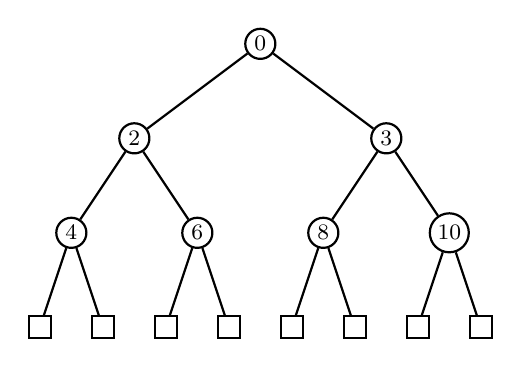
\begin{tikzpicture}
[-,thick,%
  every node/.style={shape=circle,inner sep=1.5pt,draw,thick},%
  scale=0.8]
\footnotesize
\node {$0$}
  [sibling distance=4cm]
  child {node {$2$}
    [sibling distance=2cm]
    child {node {$4$}
      [sibling distance=1cm]
      child {node[rectangle,inner sep=4pt,draw,thick] {}}
      child {node[rectangle,inner sep=4pt,draw,thick] {}}
    }
    child {node {$6$}
      [sibling distance=1cm]
      child {node[rectangle,inner sep=4pt,draw,thick] {}}
      child {node[rectangle,inner sep=4pt,draw,thick] {}}
    }
  }
  child {node {$3$}
    [sibling distance=2cm]
    child {node {$8$}
      [sibling distance=1cm]
      child {node[rectangle,inner sep=4pt,draw,thick] {}}
      child {node[rectangle,inner sep=4pt,draw,thick] {}}
    }
    child {node {$10$}
      [sibling distance=1cm]
      child {node[rectangle,inner sep=4pt,draw,thick] {}}
      child {node[rectangle,inner sep=4pt,draw,thick] {}}
    }
  };
\end{tikzpicture}
}
%%
%%
\subfigure[]{
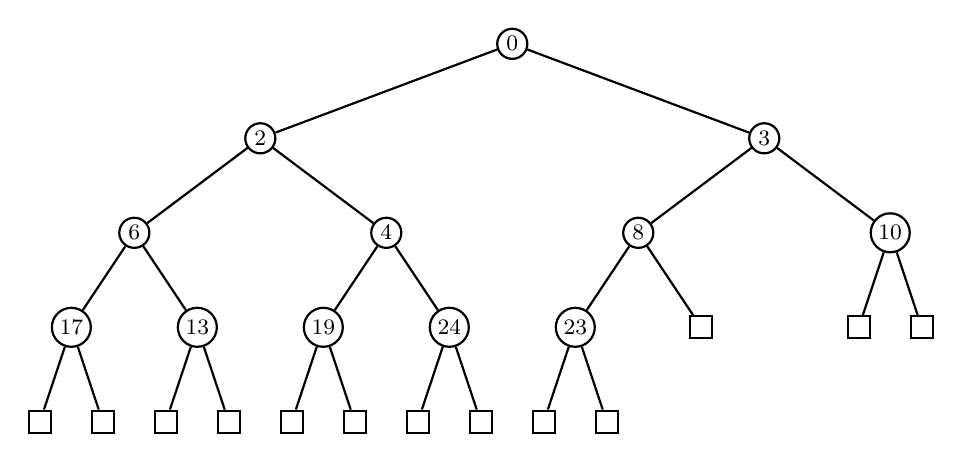
\begin{tikzpicture}
[-,thick,%
  every node/.style={shape=circle,inner sep=1.5pt,draw,thick},%
  scale=0.8]
\footnotesize
\node {$0$}
  [sibling distance=8cm]
  child {node {$2$}
    [sibling distance=4cm]
    child {node {$6$}
      [sibling distance=2cm]
      child {node {$17$}
        [sibling distance=1cm]
        child {node[rectangle,inner sep=4pt,draw,thick] {}}
        child {node[rectangle,inner sep=4pt,draw,thick] {}}
      }
      child {node {$13$}
        [sibling distance=1cm]
        child {node[rectangle,inner sep=4pt,draw,thick] {}}
        child {node[rectangle,inner sep=4pt,draw,thick] {}}
      }
    }
    child {node {$4$}
      [sibling distance=2cm]
      child {node {$19$}
        [sibling distance=1cm]
        child {node[rectangle,inner sep=4pt,draw,thick] {}}
        child {node[rectangle,inner sep=4pt,draw,thick] {}}
      }
      child {node {$24$}
        [sibling distance=1cm]
        child {node[rectangle,inner sep=4pt,draw,thick] {}}
        child {node[rectangle,inner sep=4pt,draw,thick] {}}
      }
    }
  }
  child {node {$3$}
    [sibling distance=4cm]
    child {node {$8$}
      [sibling distance=2cm]
      child {node {$23$}
        [sibling distance=1cm]
        child {node[rectangle,inner sep=4pt,draw,thick] {}}
        child {node[rectangle,inner sep=4pt,draw,thick] {}}
      }
      child {node[rectangle,inner sep=4pt,draw,thick] {}}
    }
    child {node {$10$}
      [sibling distance=1cm]
      child {node[rectangle,inner sep=4pt,draw,thick] {}}
      child {node[rectangle,inner sep=4pt,draw,thick] {}}
    }
  };
\end{tikzpicture}
}
%%
%%
\subfigure[]{
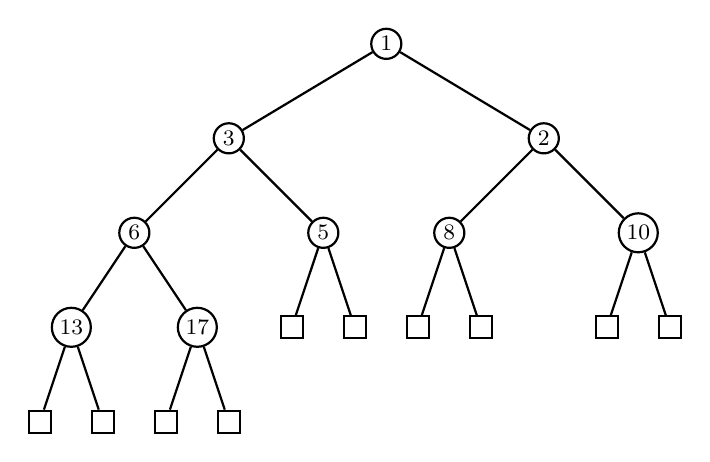
\begin{tikzpicture}
[-,thick,%
  every node/.style={shape=circle,inner sep=1.5pt,draw,thick},%
  scale=0.8]
\footnotesize
\node {$1$}
  [sibling distance=5cm]
  child {node {$3$}
    [sibling distance=3cm]
    child {node {$6$}
      [sibling distance=2cm]
      child {node {$13$}
        [sibling distance=1cm]
        child {node[rectangle,inner sep=4pt,draw,thick] {}}
        child {node[rectangle,inner sep=4pt,draw,thick] {}}
      }
      child {node {$17$}
        [sibling distance=1cm]
        child {node[rectangle,inner sep=4pt,draw,thick] {}}
        child {node[rectangle,inner sep=4pt,draw,thick] {}}
      }
    }
    child {node {$5$}
      [sibling distance=1cm]
      child {node[rectangle,inner sep=4pt,draw,thick] {}}
      child {node[rectangle,inner sep=4pt,draw,thick] {}}
    }
  }
  child {node {$2$}
    [sibling distance=3cm]
    child {node {$8$}
      [sibling distance=1cm]
      child {node[rectangle,inner sep=4pt,draw,thick] {}}
      child {node[rectangle,inner sep=4pt,draw,thick] {}}
    }
    child {node {$10$}
      [sibling distance=1cm]
      child {node[rectangle,inner sep=4pt,draw,thick] {}}
      child {node[rectangle,inner sep=4pt,draw,thick] {}}
    }
  };
\end{tikzpicture}
}
\end{figure}

\end{document}

\caption{Examples of binary heaps with integer keys.}
\label{fig:tree_data_structures:binary_heaps_integer_keys}
\end{figure}

If a binary tree $T$ satisfies both the heap-order and heap-structure
properties, then $T$ is referred to as a binary heap. By insisting
that $T$ satisfy the heap-order\index{heap-order property} property,
we are able to determine the minimum vertex of $T$ in constant time
$O(1)$. Requiring that $T$ also satisfy the
heap-structure\index{heap-structure property} property allows us to
determine the last vertex of $T$. The last vertex of $T$ is identified
as the right-most internal vertex of $T$ having the greatest depth.
Figure~\ref{fig:tree_data_structures:binary_heaps_integer_keys}
illustrates various examples of binary heaps. The heap-structure
property together with
Theorem~\ref{thm:trees_forests:complete_binary_tree_exact_order}
result in the following corollary on the height of a binary heap.

\begin{corollary}
\label{cor:tree_data_structures:height_binary_heap}
A binary heap $T$ with $n$ internal vertices has height
\[
h
=
\big\lceil \lg(n + 1) \big\rceil.\index{$\lg$}
\]
\end{corollary}

\begin{proof}
Level $h - 1$ has at least one internal vertex. Apply
Theorem~\ref{thm:trees_forests:complete_binary_tree_exact_order} to
see that $T$ has at least
\[
2^{h - 2 + 1} - 1 + 1
=
2^{h - 1}
\]
internal vertices. On the other hand, level $h - 1$ has at most
$2^{h-1}$ internal vertices. Another application of
Theorem~\ref{thm:trees_forests:complete_binary_tree_exact_order} shows
that $T$ has at most
\[
2^{h - 1 + 1} - 1
=
2^h - 1
\]
internal vertices. Thus $n$ is bounded by
\[
2^{h - 1} \leq n \leq 2^h - 1.
\]
Taking logarithms of each side in the latter bound results in
\[
\lg(n + 1) \leq h \leq \lg n + 1
\]
and the corollary follows.
\end{proof}

\begin{figure}[!htbp]
\centering
%%%%%%%%%%%%%%%%%%%%%%%%%%%%%%%%%%%%%%%%%%%%%%%%%%%%%%%%%%%%%%%%%%%%%%%%%%%
%% This file is part of the book
%%
%% Algorithmic Graph Theory
%% http://code.google.com/p/graph-theory-algorithms-book/
%%
%% Copyright (C) 2009, 2010, 2011 Minh Van Nguyen <nguyenminh2@gmail.com>
%%
%% See the file COPYING for copying conditions.
%%%%%%%%%%%%%%%%%%%%%%%%%%%%%%%%%%%%%%%%%%%%%%%%%%%%%%%%%%%%%%%%%%%%%%%%%%%

\documentclass{article}

\usepackage{subfigure}
\usepackage{tikz}
\usetikzlibrary{external}
\tikzexternalize{sample-binary-heaps-array}

\begin{document}

\begin{figure}
\subfigure[]{
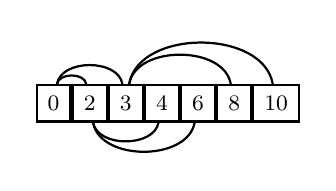
\begin{tikzpicture}
[every node/.style={inner sep=4pt,draw,thick},%
  lineDecorate/.style={-,thick}]
\footnotesize
\pgfmatrix{rectangle}{center}{}
{\pgfusepath{}}{\pgfpointorigin}{\let\&=\pgfmatrixnextcell}
{
  \node(0){$0$}; \& \node(2){$2$}; \& \node(3){$3$}; \& \node(4){$4$}; \&
  \node(6){$6$}; \& \node(8){$8$}; \& \node(10){$10$}; \\
}
\path
\foreach \startNode/\endNode/\bend in {
  0/2/bend left, 0/3/bend left, 2/4/bend right, 2/6/bend right,
  3/8/bend left, 3/10/bend left}
{
  (\startNode) edge[lineDecorate,\bend=80] (\endNode)
};
\end{tikzpicture}
}
%%
%%
\qquad
\subfigure[]{
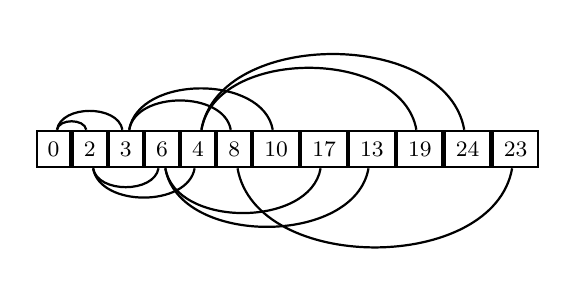
\begin{tikzpicture}
[every node/.style={inner sep=4pt,draw,thick},%
  lineDecorate/.style={-,thick}]
\footnotesize
\pgfmatrix{rectangle}{center}{}
{\pgfusepath{}}{\pgfpointorigin}{\let\&=\pgfmatrixnextcell}
{
  \node(0){$0$}; \& \node(2){$2$}; \& \node(3){$3$}; \& \node(6){$6$}; \&
  \node(4){$4$}; \& \node(8){$8$}; \& \node(10){$10$}; \& \node(17){$17$}; \&
  \node(13){$13$}; \& \node(19){$19$}; \& \node(24){$24$}; \&
  \node(23){$23$}; \\
}
\path
\foreach \startNode/\endNode/\bend in {
  0/2/bend left, 0/3/bend left, 2/6/bend right, 2/4/bend right,
  3/8/bend left, 3/10/bend left, 6/17/bend right, 6/13/bend right,
  4/19/bend left, 4/24/bend left, 8/23/bend right}
{
  (\startNode) edge[lineDecorate,\bend=80] (\endNode)
};
\end{tikzpicture}
}
%%
%%
\subfigure[]{
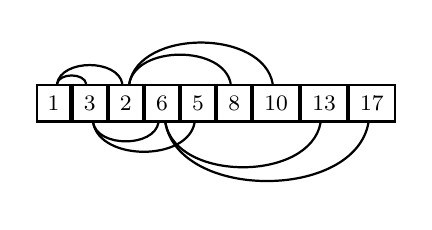
\begin{tikzpicture}
[every node/.style={inner sep=4pt,draw,thick},%
  lineDecorate/.style={-,thick}]
\footnotesize
\pgfmatrix{rectangle}{center}{}
{\pgfusepath{}}{\pgfpointorigin}{\let\&=\pgfmatrixnextcell}
{
  \node(1){$1$}; \& \node(3){$3$}; \& \node(2){$2$}; \& \node(6){$6$}; \&
  \node(5){$5$}; \& \node(8){$8$}; \& \node(10){$10$}; \&
  \node(13){$13$}; \& \node(17){$17$}; \\
}
\path
\foreach \startNode/\endNode/\bend in {
  1/3/bend left, 1/2/bend left, 3/6/bend right, 3/5/bend right,
  2/8/bend left, 2/10/bend left, 6/13/bend right, 6/17/bend right}
{
  (\startNode) edge[lineDecorate,\bend=80] (\endNode)
};
\end{tikzpicture}
}
\end{figure}

\end{document}

\caption{Sequence representations of various binary heaps.}
\label{fig:tree_data_structures:sequence_representations_binary_heaps}
\end{figure}


%%%%%%%%%%%%%%%%%%%%%%%%%%%%%%%%%%%%%%%%%%%%%%%%%%%%%%%%%%%%%%%%%%%%%%%%%%%

\subsection{Sequence representation}

Any binary heap can be represented as a binary tree. Each vertex in
the tree must know about its parent and its two children. However, a
more common approach is to represent a binary heap as a sequence such
as a list, array, or vector. Let $T$ be a binary heap consisting of
$n$ internal vertices and let $L$ be a list of $n$ elements. The root
vertex is represented as the list element $L[0]$. For each index $i$,
the children of $L[i]$ are $L[2i + 1]$ and $L[2i + 2]$ and the parent
of $L[i]$ is
\[
L\left[ \left\lfloor \frac{i - 1}{2} \right\rfloor \right].
\]
With a sequence representation of a binary heap, each vertex needs not
know about its parent and children. Such information can be obtained
via simple arithmetic on sequence indices. For example, the binary
heaps in
Figure~\ref{fig:tree_data_structures:binary_heaps_integer_keys} can be
represented as the corresponding lists in
Figure~\ref{fig:tree_data_structures:sequence_representations_binary_heaps}.
Note that it is not necessary to store the leaves of $T$ in the
sequence representation.


%%%%%%%%%%%%%%%%%%%%%%%%%%%%%%%%%%%%%%%%%%%%%%%%%%%%%%%%%%%%%%%%%%%%%%%%%%%

\subsection{Insertion and sift-up}
\label{subsec:tree_data_structures:insertion_sift_up}

We now consider the problem of inserting a vertex $v$ into a binary
heap $T$. If $T$ is empty, inserting a vertex simply involves the
creation of a new internal vertex. We let that new internal vertex be
$v$ and let its two children be leaves. The resulting binary heap
augmented with $v$ has exactly one internal vertex and satisfies both
the heap-order and heap-structure properties, as shown in
Figure~\ref{fig:tree_data_structures:insert_vertex_into_empty_binary_heap}.
In other words, any binary heap with one internal vertex trivially
satisfies the heap-order property.

\begin{figure}[!htbp]
\centering
\input{image/tree-data-structures/binary-heap-insert-empty.tex}
\caption{Inserting a vertex into an empty binary heap.}
\label{fig:tree_data_structures:insert_vertex_into_empty_binary_heap}
\end{figure}

Let $T$ now be a nonempty binary heap, i.e. $T$ has at least one
internal vertex, and suppose we want to insert into $T$ an internal
vertex $v$. We must identify the correct leaf of $T$ at which to
insert $v$. If the $n$ internal vertices of $T$ are
$r = v_0, v_1, \dots, v_{n-1}$, then by the sequence representation of
$T$ we can identify the last internal vertex $v_{n-1}$ in constant
time. The correct leaf at which to insert $v$ is the sequence element
immediately following $v_{n-1}$, i.e. the element at position $n$ in
the sequence representation of $T$. We replace with $v$ the leaf at
position $n$ in the sequence so that $v$ now becomes the last vertex
of $T$.

The binary heap $T$ augmented with the new last vertex $v$ satisfies
the heap-structure property, but may violate the heap-order
property. To ensure that $T$ satisfies the heap-order property, we
perform an operation on $T$ called \emph{sift-up}\index{sift-up} that
involves possibly moving $v$ up through various levels of $T$. Let
$k_v$ be the key of $v$ and let $k_{p(v)}$ be the key of $v$'s
parent. If the relation $k_{p(v)} \leq k_v$ holds, then $T$ satisfies
the heap-order property. Otherwise we swap $v$ with its parent,
effectively moving $v$ up one level to be at the position previously
occupied by its parent. The parent of $v$ is moved down one level and
now occupies the position where $v$ was previously. With $v$ in its
new position, we perform the same key comparison process with $v$'s
new parent. The key comparison and swapping continue until the
heap-order property holds for $T$. In the worst case, $v$ would become
the new root of $T$ after undergoing a number of swaps that is
proportional to the height of $T$. Therefore, inserting a new internal
vertex into $T$ can be achieved in time $O(\lg n)$.
Figure~\ref{fig:tree_data_structures:insert_sift_up_binary_heap}
illustrates the insertion of a new internal vertex into a nonempty
binary heap and the resulting sift-up operation to maintain the
heap-order property.
Algorithm~\ref{alg:tree_data_structures:binary_heap_insert} presents
pseudocode of our discussion for inserting a new internal vertex into
a nonempty binary heap. The pseudocode is adapted from
Howard~\cite{Howard2010}, which provides a C implementation of binary
heaps.

\begin{figure}[!htbp]
\centering
%%%%%%%%%%%%%%%%%%%%%%%%%%%%%%%%%%%%%%%%%%%%%%%%%%%%%%%%%%%%%%%%%%%%%%%%%%%
%% This file is part of the book
%%
%% Algorithmic Graph Theory
%% http://code.google.com/p/graph-theory-algorithms-book/
%%
%% Copyright (C) 2009, 2010 Minh Van Nguyen <nguyenminh2@gmail.com>
%%
%% See the file COPYING for copying conditions.
%%%%%%%%%%%%%%%%%%%%%%%%%%%%%%%%%%%%%%%%%%%%%%%%%%%%%%%%%%%%%%%%%%%%%%%%%%%

\subfigure[]{
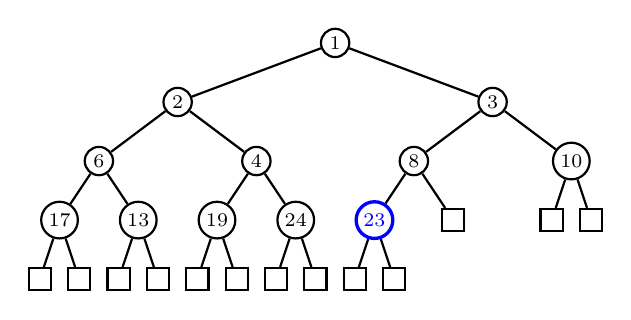
\begin{tikzpicture}
[-,thick,%
  every node/.style={shape=circle,inner sep=1.5pt,draw,thick},%
  scale=0.5]
\scriptsize
\node {$1$}
  [sibling distance=8cm]
  child {node {$2$}
    [sibling distance=4cm]
    child {node {$6$}
      [sibling distance=2cm]
      child {node {$17$}
        [sibling distance=1cm]
        child {node[rectangle,inner sep=4pt,draw,thick] {}}
        child {node[rectangle,inner sep=4pt,draw,thick] {}}
      }
      child {node {$13$}
        [sibling distance=1cm]
        child {node[rectangle,inner sep=4pt,draw,thick] {}}
        child {node[rectangle,inner sep=4pt,draw,thick] {}}
      }
    }
    child {node {$4$}
      [sibling distance=2cm]
      child {node {$19$}
        [sibling distance=1cm]
        child {node[rectangle,inner sep=4pt,draw,thick] {}}
        child {node[rectangle,inner sep=4pt,draw,thick] {}}
      }
      child {node {$24$}
        [sibling distance=1cm]
        child {node[rectangle,inner sep=4pt,draw,thick] {}}
        child {node[rectangle,inner sep=4pt,draw,thick] {}}
      }
    }
  }
  child {node {$3$}
    [sibling distance=4cm]
    child {node {$8$}
      [sibling distance=2cm]
      child {node[blue,very thick] {$23$}
        [sibling distance=1cm]
        child {node[rectangle,inner sep=4pt,draw,thick] {}}
        child {node[rectangle,inner sep=4pt,draw,thick] {}}
      }
      child {node[rectangle,inner sep=4pt,draw,thick] {}}
    }
    child {node {$10$}
      [sibling distance=1cm]
      child {node[rectangle,inner sep=4pt,draw,thick] {}}
      child {node[rectangle,inner sep=4pt,draw,thick] {}}
    }
  };
\end{tikzpicture}
}
%%
%%
\quad
\subfigure[]{
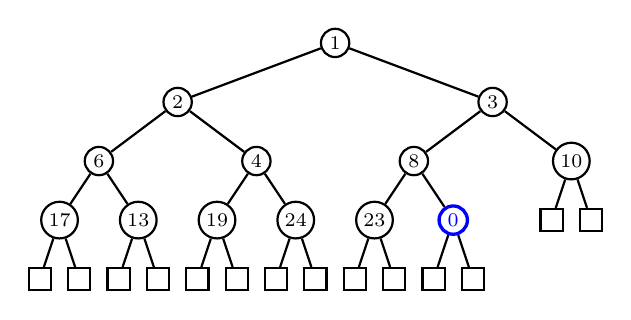
\begin{tikzpicture}
[-,thick,%
  every node/.style={shape=circle,inner sep=1.5pt,draw,thick},%
  scale=0.5]
\scriptsize
\node {$1$}
  [sibling distance=8cm]
  child {node {$2$}
    [sibling distance=4cm]
    child {node {$6$}
      [sibling distance=2cm]
      child {node {$17$}
        [sibling distance=1cm]
        child {node[rectangle,inner sep=4pt,draw,thick] {}}
        child {node[rectangle,inner sep=4pt,draw,thick] {}}
      }
      child {node {$13$}
        [sibling distance=1cm]
        child {node[rectangle,inner sep=4pt,draw,thick] {}}
        child {node[rectangle,inner sep=4pt,draw,thick] {}}
      }
    }
    child {node {$4$}
      [sibling distance=2cm]
      child {node {$19$}
        [sibling distance=1cm]
        child {node[rectangle,inner sep=4pt,draw,thick] {}}
        child {node[rectangle,inner sep=4pt,draw,thick] {}}
      }
      child {node {$24$}
        [sibling distance=1cm]
        child {node[rectangle,inner sep=4pt,draw,thick] {}}
        child {node[rectangle,inner sep=4pt,draw,thick] {}}
      }
    }
  }
  child {node {$3$}
    [sibling distance=4cm]
    child {node {$8$}
      [sibling distance=2cm]
      child {node {$23$}
        [sibling distance=1cm]
        child {node[rectangle,inner sep=4pt,draw,thick] {}}
        child {node[rectangle,inner sep=4pt,draw,thick] {}}
      }
      child {node[blue,very thick] {$0$}
        [sibling distance=1cm]
        child {node[rectangle,inner sep=4pt,draw,thick] {}}
        child {node[rectangle,inner sep=4pt,draw,thick] {}}
      }
    }
    child {node {$10$}
      [sibling distance=1cm]
      child {node[rectangle,inner sep=4pt,draw,thick] {}}
      child {node[rectangle,inner sep=4pt,draw,thick] {}}
    }
  };
\end{tikzpicture}
}
%%
%%
\subfigure[]{
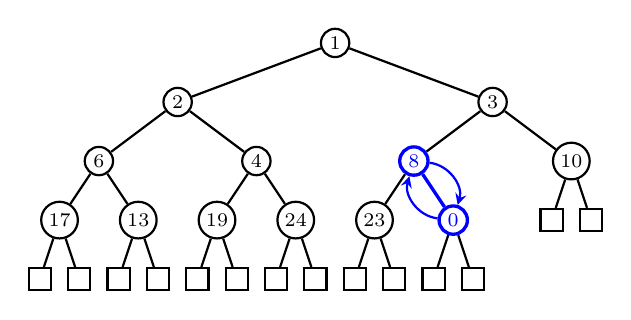
\begin{tikzpicture}
[-,thick,%
  every node/.style={shape=circle,inner sep=1.5pt,draw,thick},%
  scale=0.5]
\scriptsize
\node {$1$}
  [sibling distance=8cm]
  child {node {$2$}
    [sibling distance=4cm]
    child {node {$6$}
      [sibling distance=2cm]
      child {node {$17$}
        [sibling distance=1cm]
        child {node[rectangle,inner sep=4pt,draw,thick] {}}
        child {node[rectangle,inner sep=4pt,draw,thick] {}}
      }
      child {node {$13$}
        [sibling distance=1cm]
        child {node[rectangle,inner sep=4pt,draw,thick] {}}
        child {node[rectangle,inner sep=4pt,draw,thick] {}}
      }
    }
    child {node {$4$}
      [sibling distance=2cm]
      child {node {$19$}
        [sibling distance=1cm]
        child {node[rectangle,inner sep=4pt,draw,thick] {}}
        child {node[rectangle,inner sep=4pt,draw,thick] {}}
      }
      child {node {$24$}
        [sibling distance=1cm]
        child {node[rectangle,inner sep=4pt,draw,thick] {}}
        child {node[rectangle,inner sep=4pt,draw,thick] {}}
      }
    }
  }
  child {node {$3$}
    [sibling distance=4cm]
    child {node[blue,very thick] (8) {$8$}
      [sibling distance=2cm]
      child {node {$23$}
        [sibling distance=1cm]
        child {node[rectangle,inner sep=4pt,draw,thick] {}}
        child {node[rectangle,inner sep=4pt,draw,thick] {}}
      }
      child[blue,very thick] {node[blue,very thick] (0) {$0$}
        [sibling distance=1cm]
        child[black,thick] {node[rectangle,inner sep=4pt,draw,thick] {}}
        child[black,thick] {node[rectangle,inner sep=4pt,draw,thick] {}}
      }
    }
    child {node {$10$}
      [sibling distance=1cm]
      child {node[rectangle,inner sep=4pt,draw,thick] {}}
      child {node[rectangle,inner sep=4pt,draw,thick] {}}
    }
  };
\path
(0) edge[->,>=stealth,thick,bend left=50,blue] (8)
(8) edge[->,>=stealth,thick,bend left=50,blue] (0);
\end{tikzpicture}
}
%%
%%
\quad
\subfigure[]{
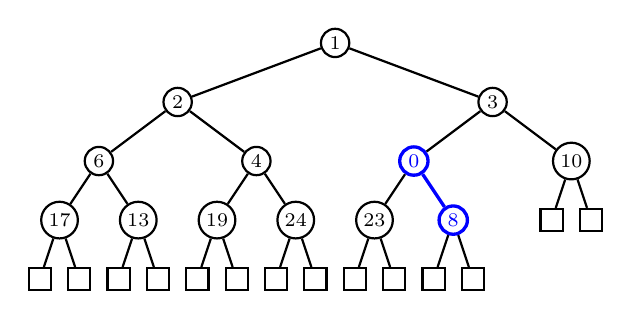
\begin{tikzpicture}
[-,thick,%
  every node/.style={shape=circle,inner sep=1.5pt,draw,thick},%
  scale=0.5]
\scriptsize
\node {$1$}
  [sibling distance=8cm]
  child {node {$2$}
    [sibling distance=4cm]
    child {node {$6$}
      [sibling distance=2cm]
      child {node {$17$}
        [sibling distance=1cm]
        child {node[rectangle,inner sep=4pt,draw,thick] {}}
        child {node[rectangle,inner sep=4pt,draw,thick] {}}
      }
      child {node {$13$}
        [sibling distance=1cm]
        child {node[rectangle,inner sep=4pt,draw,thick] {}}
        child {node[rectangle,inner sep=4pt,draw,thick] {}}
      }
    }
    child {node {$4$}
      [sibling distance=2cm]
      child {node {$19$}
        [sibling distance=1cm]
        child {node[rectangle,inner sep=4pt,draw,thick] {}}
        child {node[rectangle,inner sep=4pt,draw,thick] {}}
      }
      child {node {$24$}
        [sibling distance=1cm]
        child {node[rectangle,inner sep=4pt,draw,thick] {}}
        child {node[rectangle,inner sep=4pt,draw,thick] {}}
      }
    }
  }
  child {node {$3$}
    [sibling distance=4cm]
    child {node[blue,very thick] {$0$}
      [sibling distance=2cm]
      child {node {$23$}
        [sibling distance=1cm]
        child {node[rectangle,inner sep=4pt,draw,thick] {}}
        child {node[rectangle,inner sep=4pt,draw,thick] {}}
      }
      child[blue,very thick] {node[blue,very thick] {$8$}
        [sibling distance=1cm]
        child[black,thick] {node[rectangle,inner sep=4pt,draw,thick] {}}
        child[black,thick] {node[rectangle,inner sep=4pt,draw,thick] {}}
      }
    }
    child {node {$10$}
      [sibling distance=1cm]
      child {node[rectangle,inner sep=4pt,draw,thick] {}}
      child {node[rectangle,inner sep=4pt,draw,thick] {}}
    }
  };
\end{tikzpicture}
}
%%
%%
\subfigure[]{
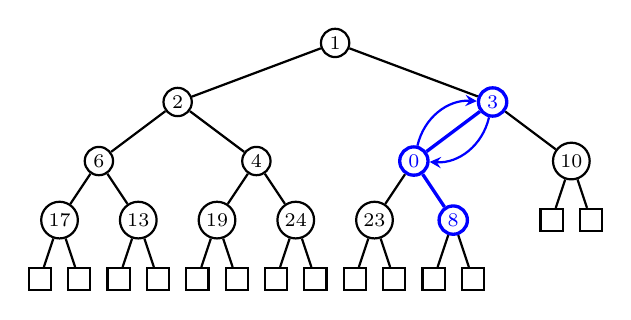
\begin{tikzpicture}
[-,thick,%
  every node/.style={shape=circle,inner sep=1.5pt,draw,thick},%
  scale=0.5]
\scriptsize
\node {$1$}
  [sibling distance=8cm]
  child {node {$2$}
    [sibling distance=4cm]
    child {node {$6$}
      [sibling distance=2cm]
      child {node {$17$}
        [sibling distance=1cm]
        child {node[rectangle,inner sep=4pt,draw,thick] {}}
        child {node[rectangle,inner sep=4pt,draw,thick] {}}
      }
      child {node {$13$}
        [sibling distance=1cm]
        child {node[rectangle,inner sep=4pt,draw,thick] {}}
        child {node[rectangle,inner sep=4pt,draw,thick] {}}
      }
    }
    child {node {$4$}
      [sibling distance=2cm]
      child {node {$19$}
        [sibling distance=1cm]
        child {node[rectangle,inner sep=4pt,draw,thick] {}}
        child {node[rectangle,inner sep=4pt,draw,thick] {}}
      }
      child {node {$24$}
        [sibling distance=1cm]
        child {node[rectangle,inner sep=4pt,draw,thick] {}}
        child {node[rectangle,inner sep=4pt,draw,thick] {}}
      }
    }
  }
  child {node[blue,very thick] (3) {$3$}
    [sibling distance=4cm]
    child[blue,very thick] {node[blue,very thick] (0) {$0$}
      [sibling distance=2cm]
      child[black,thick] {node {$23$}
        [sibling distance=1cm]
        child {node[rectangle,inner sep=4pt,draw,thick] {}}
        child {node[rectangle,inner sep=4pt,draw,thick] {}}
      }
      child[blue,very thick] {node[blue,very thick] {$8$}
        [sibling distance=1cm]
        child[black,thick] {node[rectangle,inner sep=4pt,draw,thick] {}}
        child[black,thick] {node[rectangle,inner sep=4pt,draw,thick] {}}
      }
    }
    child {node {$10$}
      [sibling distance=1cm]
      child {node[rectangle,inner sep=4pt,draw,thick] {}}
      child {node[rectangle,inner sep=4pt,draw,thick] {}}
    }
  };
\path
(0) edge[->,>=stealth,thick,bend left=40,blue] (3)
(3) edge[->,>=stealth,thick,bend left=40,blue] (0);
\end{tikzpicture}
}
%%
%%
\quad
\subfigure[]{
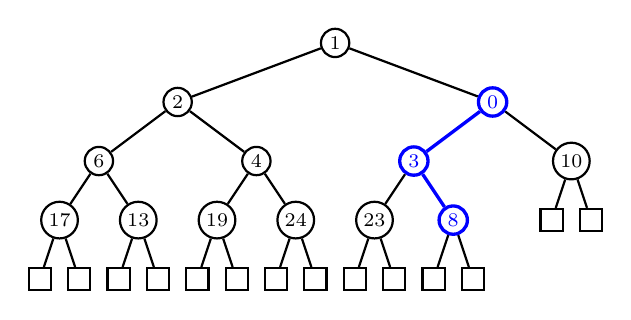
\begin{tikzpicture}
[-,thick,%
  every node/.style={shape=circle,inner sep=1.5pt,draw,thick},%
  scale=0.5]
\scriptsize
\node {$1$}
  [sibling distance=8cm]
  child {node {$2$}
    [sibling distance=4cm]
    child {node {$6$}
      [sibling distance=2cm]
      child {node {$17$}
        [sibling distance=1cm]
        child {node[rectangle,inner sep=4pt,draw,thick] {}}
        child {node[rectangle,inner sep=4pt,draw,thick] {}}
      }
      child {node {$13$}
        [sibling distance=1cm]
        child {node[rectangle,inner sep=4pt,draw,thick] {}}
        child {node[rectangle,inner sep=4pt,draw,thick] {}}
      }
    }
    child {node {$4$}
      [sibling distance=2cm]
      child {node {$19$}
        [sibling distance=1cm]
        child {node[rectangle,inner sep=4pt,draw,thick] {}}
        child {node[rectangle,inner sep=4pt,draw,thick] {}}
      }
      child {node {$24$}
        [sibling distance=1cm]
        child {node[rectangle,inner sep=4pt,draw,thick] {}}
        child {node[rectangle,inner sep=4pt,draw,thick] {}}
      }
    }
  }
  child {node[blue,very thick] {$0$}
    [sibling distance=4cm]
    child[blue,very thick] {node[blue,very thick] {$3$}
      [sibling distance=2cm]
      child[black,thick] {node {$23$}
        [sibling distance=1cm]
        child {node[rectangle,inner sep=4pt,draw,thick] {}}
        child {node[rectangle,inner sep=4pt,draw,thick] {}}
      }
      child[blue,very thick] {node[blue,very thick] {$8$}
        [sibling distance=1cm]
        child[black,thick] {node[rectangle,inner sep=4pt,draw,thick] {}}
        child[black,thick] {node[rectangle,inner sep=4pt,draw,thick] {}}
      }
    }
    child {node {$10$}
      [sibling distance=1cm]
      child {node[rectangle,inner sep=4pt,draw,thick] {}}
      child {node[rectangle,inner sep=4pt,draw,thick] {}}
    }
  };
\end{tikzpicture}
}
%%
%%
\subfigure[]{
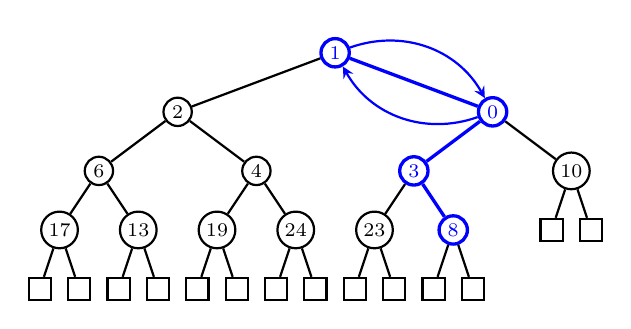
\begin{tikzpicture}
[-,thick,%
  every node/.style={shape=circle,inner sep=1.5pt,draw,thick},%
  scale=0.5]
\scriptsize
\node[blue,very thick] (1) {$1$}
  [sibling distance=8cm]
  child {node {$2$}
    [sibling distance=4cm]
    child {node {$6$}
      [sibling distance=2cm]
      child {node {$17$}
        [sibling distance=1cm]
        child {node[rectangle,inner sep=4pt,draw,thick] {}}
        child {node[rectangle,inner sep=4pt,draw,thick] {}}
      }
      child {node {$13$}
        [sibling distance=1cm]
        child {node[rectangle,inner sep=4pt,draw,thick] {}}
        child {node[rectangle,inner sep=4pt,draw,thick] {}}
      }
    }
    child {node {$4$}
      [sibling distance=2cm]
      child {node {$19$}
        [sibling distance=1cm]
        child {node[rectangle,inner sep=4pt,draw,thick] {}}
        child {node[rectangle,inner sep=4pt,draw,thick] {}}
      }
      child {node {$24$}
        [sibling distance=1cm]
        child {node[rectangle,inner sep=4pt,draw,thick] {}}
        child {node[rectangle,inner sep=4pt,draw,thick] {}}
      }
    }
  }
  child[blue,very thick] {node[blue,very thick] (0) {$0$}
    [sibling distance=4cm]
    child[blue,very thick] {node[blue,very thick] {$3$}
      [sibling distance=2cm]
      child[black,thick] {node {$23$}
        [sibling distance=1cm]
        child {node[rectangle,inner sep=4pt,draw,thick] {}}
        child {node[rectangle,inner sep=4pt,draw,thick] {}}
      }
      child[blue,very thick] {node[blue,very thick] {$8$}
        [sibling distance=1cm]
        child[black,thick] {node[rectangle,inner sep=4pt,draw,thick] {}}
        child[black,thick] {node[rectangle,inner sep=4pt,draw,thick] {}}
      }
    }
    child[black,thick] {node {$10$}
      [sibling distance=1cm]
      child {node[rectangle,inner sep=4pt,draw,thick] {}}
      child {node[rectangle,inner sep=4pt,draw,thick] {}}
    }
  };
\path
(0) edge[->,>=stealth,thick,bend left=40,blue] (1)
(1) edge[->,>=stealth,thick,bend left=40,blue] (0);
\end{tikzpicture}
}
%%
%%
\quad
\subfigure[]{
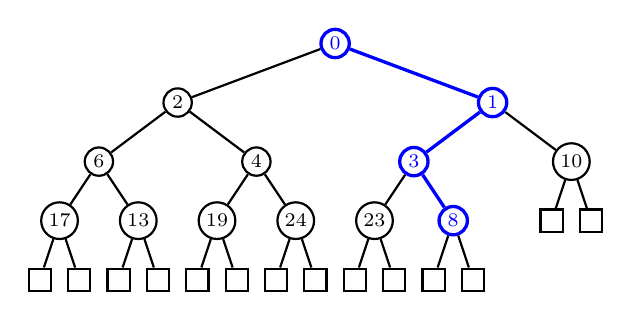
\begin{tikzpicture}
[-,thick,%
  every node/.style={shape=circle,inner sep=1.5pt,draw,thick},%
  scale=0.5]
\scriptsize
\node[blue,very thick] {$0$}
  [sibling distance=8cm]
  child {node {$2$}
    [sibling distance=4cm]
    child {node {$6$}
      [sibling distance=2cm]
      child {node {$17$}
        [sibling distance=1cm]
        child {node[rectangle,inner sep=4pt,draw,thick] {}}
        child {node[rectangle,inner sep=4pt,draw,thick] {}}
      }
      child {node {$13$}
        [sibling distance=1cm]
        child {node[rectangle,inner sep=4pt,draw,thick] {}}
        child {node[rectangle,inner sep=4pt,draw,thick] {}}
      }
    }
    child {node {$4$}
      [sibling distance=2cm]
      child {node {$19$}
        [sibling distance=1cm]
        child {node[rectangle,inner sep=4pt,draw,thick] {}}
        child {node[rectangle,inner sep=4pt,draw,thick] {}}
      }
      child {node {$24$}
        [sibling distance=1cm]
        child {node[rectangle,inner sep=4pt,draw,thick] {}}
        child {node[rectangle,inner sep=4pt,draw,thick] {}}
      }
    }
  }
  child[blue,very thick] {node[blue,very thick] {$1$}
    [sibling distance=4cm]
    child[blue,very thick] {node[blue,very thick] {$3$}
      [sibling distance=2cm]
      child[black,thick] {node {$23$}
        [sibling distance=1cm]
        child {node[rectangle,inner sep=4pt,draw,thick] {}}
        child {node[rectangle,inner sep=4pt,draw,thick] {}}
      }
      child[blue,very thick] {node[blue,very thick] {$8$}
        [sibling distance=1cm]
        child[black,thick] {node[rectangle,inner sep=4pt,draw,thick] {}}
        child[black,thick] {node[rectangle,inner sep=4pt,draw,thick] {}}
      }
    }
    child[black,thick] {node {$10$}
      [sibling distance=1cm]
      child {node[rectangle,inner sep=4pt,draw,thick] {}}
      child {node[rectangle,inner sep=4pt,draw,thick] {}}
    }
  };
\end{tikzpicture}
}

\caption{Insert and sift-up in a binary heap.}
\label{fig:tree_data_structures:insert_sift_up_binary_heap}
\end{figure}

\begin{algorithm}[!htbp]
%%%%%%%%%%%%%%%%%%%%%%%%%%%%%%%%%%%%%%%%%%%%%%%%%%%%%%%%%%%%%%%%%%%%%%%%%%%
%% This file is part of the book
%%
%% Algorithmic Graph Theory
%% http://code.google.com/p/graph-theory-algorithms-book/
%%
%% Copyright (C) 2009, 2010 Minh Van Nguyen <nguyenminh2@gmail.com>
%%
%% See the file COPYING for copying conditions.
%%%%%%%%%%%%%%%%%%%%%%%%%%%%%%%%%%%%%%%%%%%%%%%%%%%%%%%%%%%%%%%%%%%%%%%%%%%

\DontPrintSemicolon
\SetAlgoNoLine
%%
%% data section
\SetKwInOut{Input}{Input}
\SetKwInOut{Output}{Output}
%%
%% input/output
\Input{A nonempty binary heap $T$, in sequence representation, having
  $n$ internal vertices. An element $v$ that is to be inserted as a
  new internal vertex of $T$.}
\Output{The binary heap $T$ augmented with the new internal vertex $v$.}
\BlankLine
%%
%% algorithm body
$i \assign n$\;
\While{$i > 0$}{
  $p \assign \lfloor (i - 1) / 2\rfloor$\;
  \eIf{$\kappa_{T[p]} \leq \kappa_{v}$}{
    exit the loop\;
  }{
    $T[i] \assign T[p]$\;
    $i \assign p$\;
  }
}
$T[i] \assign v$\;
\Return $T$\;

\caption{Inserting a new internal vertex into a binary heap.}
\label{alg:tree_data_structures:binary_heap_insert}
\end{algorithm}


%%%%%%%%%%%%%%%%%%%%%%%%%%%%%%%%%%%%%%%%%%%%%%%%%%%%%%%%%%%%%%%%%%%%%%%%%%%

\subsection{Deletion and sift-down}
\label{subsec:tree_data_structures:deletion_sift_down}

The process for deleting the minimum vertex of a binary heap bears
some resemblance to that of inserting a new internal vertex into the
heap. Having removed the minimum vertex, we must then ensure that the
resulting binary heap satisfies the heap-order property. Let $T$ be a
binary heap. By the heap-order property, the root of $T$ has a key
that is minimum among all keys of internal vertices in $T$. If the
root $r$ of $T$ is the only internal vertex of $T$, i.e. $T$ is the
trivial binary heap, we simply remove $r$ and $T$ now becomes the
empty binary heap or the trivial tree, for which the heap-order
property vacuously holds.
Figure~\ref{fig:tree_data_structures:deleting_root_trivial_binary_heap}
illustrates the case of removing the root of a binary heap having one
internal vertex.

\begin{figure}[!htbp]
\centering
%%%%%%%%%%%%%%%%%%%%%%%%%%%%%%%%%%%%%%%%%%%%%%%%%%%%%%%%%%%%%%%%%%%%%%%%%%%
%% This file is part of the book
%%
%% Algorithmic Graph Theory
%% http://code.google.com/p/graph-theory-algorithms-book/
%%
%% Copyright (C) 2009, 2010, 2011 Minh Van Nguyen <nguyenminh2@gmail.com>
%%
%% See the file COPYING for copying conditions.
%%%%%%%%%%%%%%%%%%%%%%%%%%%%%%%%%%%%%%%%%%%%%%%%%%%%%%%%%%%%%%%%%%%%%%%%%%%

\documentclass{article}

\usepackage{subfigure}
\usepackage{tikz}
\usetikzlibrary{external}
\usetikzlibrary{trees}
\tikzexternalize{binary-heap-delete-empty}

\begin{document}

\begin{figure}
\subfigure[]{
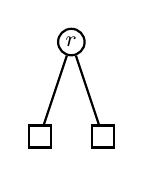
\begin{tikzpicture}
[-,thick,%
  every node/.style={shape=circle,inner sep=1.5pt,draw,thick},%
  scale=0.8]
\footnotesize
\node {$r$}
  [sibling distance=1cm]
  child {node[rectangle,inner sep=4pt,draw,thick] {}}
  child {node[rectangle,inner sep=4pt,draw,thick] {}};
\end{tikzpicture}
}
%%
%%
\qquad
\subfigure[]{
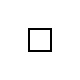
\begin{tikzpicture}
[-,thick,%
  every node/.style={shape=rectangle,inner sep=4pt,draw,thick},%
  scale=0.8]
\footnotesize
\node {};
\end{tikzpicture}
}
\end{figure}

\end{document}

\caption{Deleting the root of a trivial binary heap.}
\label{fig:tree_data_structures:deleting_root_trivial_binary_heap}
\end{figure}

We now turn to the case where $T$ has $n > 1$ internal vertices. Let
$r$ be the root of $T$ and let $v$ be the last internal vertex of
$T$. Deleting $r$ would disconnect $T$. So we instead replace the key
and information at $r$ with the key and other relevant information
pertaining to $v$. The root $r$ now has the key of the last internal
vertex, and $v$ becomes a leaf.

At this point, $T$ satisfies the heap-structure property but may
violate the heap-order property. To restore the heap-order property,
we perform an operation on $T$ called
\emph{sift-down}\index{sift-down} that may possibly move $r$ down
through various levels of $T$. Let $c(r)$ be the child of $r$ with key
that is minimum among all the children of $r$, and let $k_r$ and
$k_{c(r)}$ be the keys of $r$ and $c(r)$, respectively. If
$k_r \leq k_{c(r)}$, then the heap-order property is
satisfied. Otherwise we swap $r$ with $c(r)$, moving $r$ down one
level to the position previously occupied by $c(r)$. Furthermore,
$c(r)$ is moved up one level to the position previously occupied by
$r$. With $r$ in its new position, we perform the same key comparison
process with a child of $r$ that has minimum key among all of $r$'s
children. The key comparison and swapping continue until the
heap-order property holds for $T$. In the worst case, $r$ would
percolate all the way down to the level that is immediately above the
last level after undergoing a number of swaps that is proportional to
the height of $T$. Therefore, deleting the minimum vertex of $T$ can
be achieved in time $O(\lg n)$.
Figure~\ref{fig:tree_data_structures:delete_sift_down_binary_heap}
illustrates the deletion of the minimum vertex of a binary heap with
at least two internal vertices and the resulting sift-down process
that percolates vertices down through various levels of the heap in
order to maintain the heap-order
property. Algorithm~\ref{alg:tree_data_structures:binary_heap_delete}
summarizes our discussion of the process for extracting the minimum
vertex of $T$ while also ensuring that $T$ satisfies the heap-order
property. The pseudocode is adapted from the C implementation of
binary heaps in Howard~\cite{Howard2010}. With some minor changes,
Algorithm~\ref{alg:tree_data_structures:binary_heap_delete} can be
used to change the key of the root vertex and maintain the heap-order
property for the resulting binary tree.

\begin{figure}[!htbp]
\centering
%%%%%%%%%%%%%%%%%%%%%%%%%%%%%%%%%%%%%%%%%%%%%%%%%%%%%%%%%%%%%%%%%%%%%%%%%%%
%% This file is part of the book
%%
%% Algorithmic Graph Theory
%% http://code.google.com/p/graph-theory-algorithms-book/
%%
%% Copyright (C) 2009, 2010, 2011 Minh Van Nguyen <nguyenminh2@gmail.com>
%%
%% See the file COPYING for copying conditions.
%%%%%%%%%%%%%%%%%%%%%%%%%%%%%%%%%%%%%%%%%%%%%%%%%%%%%%%%%%%%%%%%%%%%%%%%%%%

\subfigure[]{
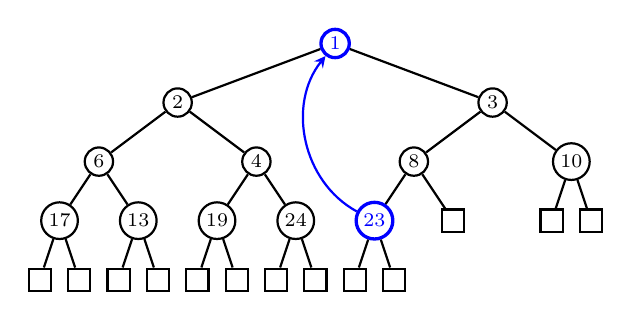
\begin{tikzpicture}
[-,thick,%
  every node/.style={shape=circle,inner sep=1.5pt,draw,thick},%
  scale=0.5]
\scriptsize
\node[blue,very thick] (1) {$1$}
  [sibling distance=8cm]
  child {node {$2$}
    [sibling distance=4cm]
    child {node {$6$}
      [sibling distance=2cm]
      child {node {$17$}
        [sibling distance=1cm]
        child {node[rectangle,inner sep=4pt,draw,thick] {}}
        child {node[rectangle,inner sep=4pt,draw,thick] {}}
      }
      child {node {$13$}
        [sibling distance=1cm]
        child {node[rectangle,inner sep=4pt,draw,thick] {}}
        child {node[rectangle,inner sep=4pt,draw,thick] {}}
      }
    }
    child {node {$4$}
      [sibling distance=2cm]
      child {node {$19$}
        [sibling distance=1cm]
        child {node[rectangle,inner sep=4pt,draw,thick] {}}
        child {node[rectangle,inner sep=4pt,draw,thick] {}}
      }
      child {node {$24$}
        [sibling distance=1cm]
        child {node[rectangle,inner sep=4pt,draw,thick] {}}
        child {node[rectangle,inner sep=4pt,draw,thick] {}}
      }
    }
  }
  child {node {$3$}
    [sibling distance=4cm]
    child {node {$8$}
      [sibling distance=2cm]
      child {node[blue,very thick] (23) {$23$}
        [sibling distance=1cm]
        child {node[rectangle,inner sep=4pt,draw,thick] {}}
        child {node[rectangle,inner sep=4pt,draw,thick] {}}
      }
      child {node[rectangle,inner sep=4pt,draw,thick] {}}
    }
    child {node {$10$}
      [sibling distance=1cm]
      child {node[rectangle,inner sep=4pt,draw,thick] {}}
      child {node[rectangle,inner sep=4pt,draw,thick] {}}
    }
  };
\path
(23) edge[->,>=stealth,thick,bend left=50,blue] (1);
\end{tikzpicture}
}
%%
%%
\quad
\subfigure[]{
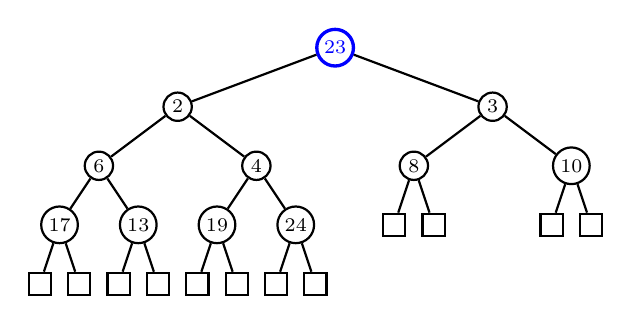
\begin{tikzpicture}
[-,thick,%
  every node/.style={shape=circle,inner sep=1.5pt,draw,thick},%
  scale=0.5]
\scriptsize
\node[blue,very thick] {$23$}
  [sibling distance=8cm]
  child {node {$2$}
    [sibling distance=4cm]
    child {node {$6$}
      [sibling distance=2cm]
      child {node {$17$}
        [sibling distance=1cm]
        child {node[rectangle,inner sep=4pt,draw,thick] {}}
        child {node[rectangle,inner sep=4pt,draw,thick] {}}
      }
      child {node {$13$}
        [sibling distance=1cm]
        child {node[rectangle,inner sep=4pt,draw,thick] {}}
        child {node[rectangle,inner sep=4pt,draw,thick] {}}
      }
    }
    child {node {$4$}
      [sibling distance=2cm]
      child {node {$19$}
        [sibling distance=1cm]
        child {node[rectangle,inner sep=4pt,draw,thick] {}}
        child {node[rectangle,inner sep=4pt,draw,thick] {}}
      }
      child {node {$24$}
        [sibling distance=1cm]
        child {node[rectangle,inner sep=4pt,draw,thick] {}}
        child {node[rectangle,inner sep=4pt,draw,thick] {}}
      }
    }
  }
  child {node {$3$}
    [sibling distance=4cm]
    child {node {$8$}
      [sibling distance=1cm]
      child {node[rectangle,inner sep=4pt,draw,thick] {}}
      child {node[rectangle,inner sep=4pt,draw,thick] {}}
    }
    child {node {$10$}
      [sibling distance=1cm]
      child {node[rectangle,inner sep=4pt,draw,thick] {}}
      child {node[rectangle,inner sep=4pt,draw,thick] {}}
    }
  };
\end{tikzpicture}
}
%%
%%
\subfigure[]{
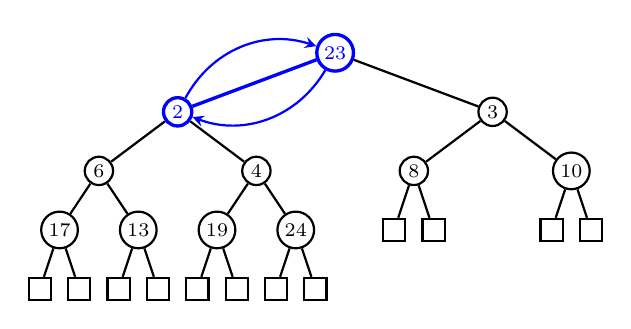
\begin{tikzpicture}
[-,thick,%
  every node/.style={shape=circle,inner sep=1.5pt,draw,thick},%
  scale=0.5]
\scriptsize
\node[blue,very thick] (23) {$23$}
  [sibling distance=8cm]
  child[blue,very thick] {node[blue,very thick] (2) {$2$}
    [sibling distance=4cm]
    child[black,thick] {node {$6$}
      [sibling distance=2cm]
      child {node {$17$}
        [sibling distance=1cm]
        child {node[rectangle,inner sep=4pt,draw,thick] {}}
        child {node[rectangle,inner sep=4pt,draw,thick] {}}
      }
      child {node {$13$}
        [sibling distance=1cm]
        child {node[rectangle,inner sep=4pt,draw,thick] {}}
        child {node[rectangle,inner sep=4pt,draw,thick] {}}
      }
    }
    child[black,thick] {node {$4$}
      [sibling distance=2cm]
      child {node {$19$}
        [sibling distance=1cm]
        child {node[rectangle,inner sep=4pt,draw,thick] {}}
        child {node[rectangle,inner sep=4pt,draw,thick] {}}
      }
      child {node {$24$}
        [sibling distance=1cm]
        child {node[rectangle,inner sep=4pt,draw,thick] {}}
        child {node[rectangle,inner sep=4pt,draw,thick] {}}
      }
    }
  }
  child {node {$3$}
    [sibling distance=4cm]
    child {node {$8$}
      [sibling distance=1cm]
      child {node[rectangle,inner sep=4pt,draw,thick] {}}
      child {node[rectangle,inner sep=4pt,draw,thick] {}}
    }
    child {node {$10$}
      [sibling distance=1cm]
      child {node[rectangle,inner sep=4pt,draw,thick] {}}
      child {node[rectangle,inner sep=4pt,draw,thick] {}}
    }
  };
\path
(2) edge[->,>=stealth,thick,bend left=40,blue] (23)
(23) edge[->,>=stealth,thick,bend left=40,blue] (2);
\end{tikzpicture}
}
%%
%%
\quad
\subfigure[]{
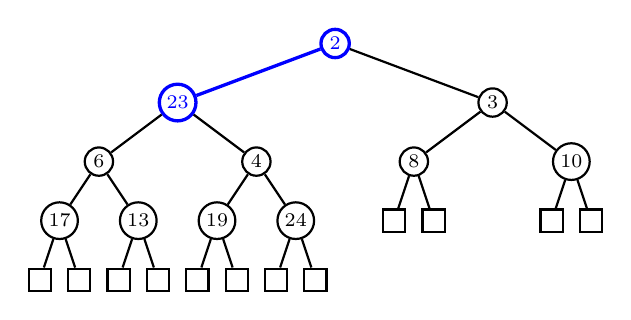
\begin{tikzpicture}
[-,thick,%
  every node/.style={shape=circle,inner sep=1.5pt,draw,thick},%
  scale=0.5]
\scriptsize
\node[blue,very thick] {$2$}
  [sibling distance=8cm]
  child[blue,very thick] {node[blue,very thick] {$23$}
    [sibling distance=4cm]
    child[black,thick] {node {$6$}
      [sibling distance=2cm]
      child {node {$17$}
        [sibling distance=1cm]
        child {node[rectangle,inner sep=4pt,draw,thick] {}}
        child {node[rectangle,inner sep=4pt,draw,thick] {}}
      }
      child {node {$13$}
        [sibling distance=1cm]
        child {node[rectangle,inner sep=4pt,draw,thick] {}}
        child {node[rectangle,inner sep=4pt,draw,thick] {}}
      }
    }
    child[black,thick] {node {$4$}
      [sibling distance=2cm]
      child {node {$19$}
        [sibling distance=1cm]
        child {node[rectangle,inner sep=4pt,draw,thick] {}}
        child {node[rectangle,inner sep=4pt,draw,thick] {}}
      }
      child {node {$24$}
        [sibling distance=1cm]
        child {node[rectangle,inner sep=4pt,draw,thick] {}}
        child {node[rectangle,inner sep=4pt,draw,thick] {}}
      }
    }
  }
  child {node {$3$}
    [sibling distance=4cm]
    child {node {$8$}
      [sibling distance=1cm]
      child {node[rectangle,inner sep=4pt,draw,thick] {}}
      child {node[rectangle,inner sep=4pt,draw,thick] {}}
    }
    child {node {$10$}
      [sibling distance=1cm]
      child {node[rectangle,inner sep=4pt,draw,thick] {}}
      child {node[rectangle,inner sep=4pt,draw,thick] {}}
    }
  };
\end{tikzpicture}
}
%%
%%
\subfigure[]{
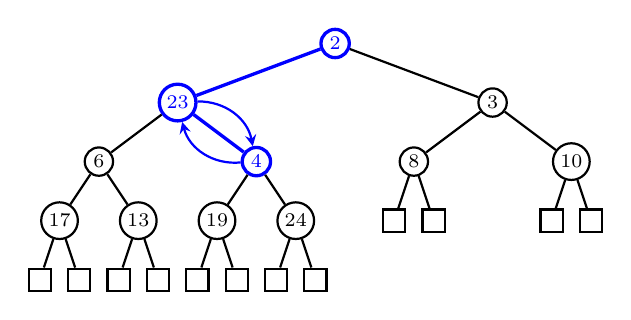
\begin{tikzpicture}
[-,thick,%
  every node/.style={shape=circle,inner sep=1.5pt,draw,thick},%
  scale=0.5]
\scriptsize
\node[blue,very thick] {$2$}
  [sibling distance=8cm]
  child[blue,very thick] {node[blue,very thick] (23) {$23$}
    [sibling distance=4cm]
    child[black,thick] {node {$6$}
      [sibling distance=2cm]
      child {node {$17$}
        [sibling distance=1cm]
        child {node[rectangle,inner sep=4pt,draw,thick] {}}
        child {node[rectangle,inner sep=4pt,draw,thick] {}}
      }
      child {node {$13$}
        [sibling distance=1cm]
        child {node[rectangle,inner sep=4pt,draw,thick] {}}
        child {node[rectangle,inner sep=4pt,draw,thick] {}}
      }
    }
    child[blue,very thick] {node[blue,very thick] (4) {$4$}
      [sibling distance=2cm]
      child[black,thick] {node {$19$}
        [sibling distance=1cm]
        child {node[rectangle,inner sep=4pt,draw,thick] {}}
        child {node[rectangle,inner sep=4pt,draw,thick] {}}
      }
      child[black,thick] {node {$24$}
        [sibling distance=1cm]
        child {node[rectangle,inner sep=4pt,draw,thick] {}}
        child {node[rectangle,inner sep=4pt,draw,thick] {}}
      }
    }
  }
  child {node {$3$}
    [sibling distance=4cm]
    child {node {$8$}
      [sibling distance=1cm]
      child {node[rectangle,inner sep=4pt,draw,thick] {}}
      child {node[rectangle,inner sep=4pt,draw,thick] {}}
    }
    child {node {$10$}
      [sibling distance=1cm]
      child {node[rectangle,inner sep=4pt,draw,thick] {}}
      child {node[rectangle,inner sep=4pt,draw,thick] {}}
    }
  };
\path
(4) edge[->,>=stealth,thick,bend left=40,blue] (23)
(23) edge[->,>=stealth,thick,bend left=40,blue] (4);
\end{tikzpicture}
}
%%
%%
\quad
\subfigure[]{
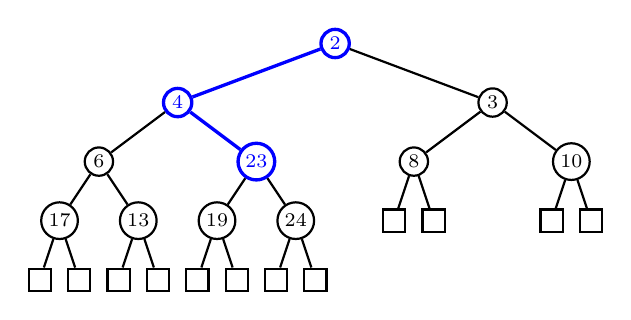
\begin{tikzpicture}
[-,thick,%
  every node/.style={shape=circle,inner sep=1.5pt,draw,thick},%
  scale=0.5]
\scriptsize
\node[blue,very thick] {$2$}
  [sibling distance=8cm]
  child[blue,very thick] {node[blue,very thick] {$4$}
    [sibling distance=4cm]
    child[black,thick] {node {$6$}
      [sibling distance=2cm]
      child {node {$17$}
        [sibling distance=1cm]
        child {node[rectangle,inner sep=4pt,draw,thick] {}}
        child {node[rectangle,inner sep=4pt,draw,thick] {}}
      }
      child {node {$13$}
        [sibling distance=1cm]
        child {node[rectangle,inner sep=4pt,draw,thick] {}}
        child {node[rectangle,inner sep=4pt,draw,thick] {}}
      }
    }
    child[blue,very thick] {node[blue,very thick] {$23$}
      [sibling distance=2cm]
      child[black,thick] {node {$19$}
        [sibling distance=1cm]
        child {node[rectangle,inner sep=4pt,draw,thick] {}}
        child {node[rectangle,inner sep=4pt,draw,thick] {}}
      }
      child[black,thick] {node {$24$}
        [sibling distance=1cm]
        child {node[rectangle,inner sep=4pt,draw,thick] {}}
        child {node[rectangle,inner sep=4pt,draw,thick] {}}
      }
    }
  }
  child {node {$3$}
    [sibling distance=4cm]
    child {node {$8$}
      [sibling distance=1cm]
      child {node[rectangle,inner sep=4pt,draw,thick] {}}
      child {node[rectangle,inner sep=4pt,draw,thick] {}}
    }
    child {node {$10$}
      [sibling distance=1cm]
      child {node[rectangle,inner sep=4pt,draw,thick] {}}
      child {node[rectangle,inner sep=4pt,draw,thick] {}}
    }
  };
\end{tikzpicture}
}
%%
%%
\subfigure[]{
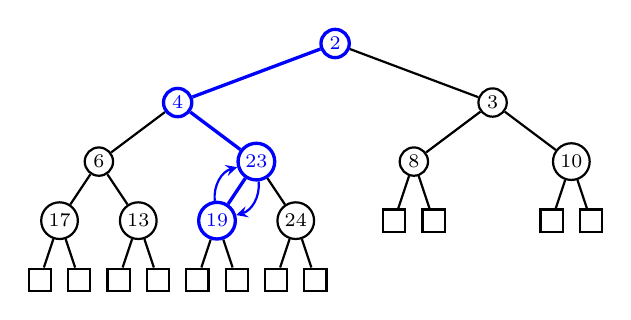
\begin{tikzpicture}
[-,thick,%
  every node/.style={shape=circle,inner sep=1.5pt,draw,thick},%
  scale=0.5]
\scriptsize
\node[blue,very thick] {$2$}
  [sibling distance=8cm]
  child[blue,very thick] {node[blue,very thick] {$4$}
    [sibling distance=4cm]
    child[black,thick] {node {$6$}
      [sibling distance=2cm]
      child {node {$17$}
        [sibling distance=1cm]
        child {node[rectangle,inner sep=4pt,draw,thick] {}}
        child {node[rectangle,inner sep=4pt,draw,thick] {}}
      }
      child {node {$13$}
        [sibling distance=1cm]
        child {node[rectangle,inner sep=4pt,draw,thick] {}}
        child {node[rectangle,inner sep=4pt,draw,thick] {}}
      }
    }
    child[blue,very thick] {node[blue,very thick] (23) {$23$}
      [sibling distance=2cm]
      child[blue,very thick] {node[blue,very thick] (19) {$19$}
        [sibling distance=1cm]
        child[black,thick] {node[rectangle,inner sep=4pt,draw,thick] {}}
        child[black,thick] {node[rectangle,inner sep=4pt,draw,thick] {}}
      }
      child[black,thick] {node {$24$}
        [sibling distance=1cm]
        child {node[rectangle,inner sep=4pt,draw,thick] {}}
        child {node[rectangle,inner sep=4pt,draw,thick] {}}
      }
    }
  }
  child {node {$3$}
    [sibling distance=4cm]
    child {node {$8$}
      [sibling distance=1cm]
      child {node[rectangle,inner sep=4pt,draw,thick] {}}
      child {node[rectangle,inner sep=4pt,draw,thick] {}}
    }
    child {node {$10$}
      [sibling distance=1cm]
      child {node[rectangle,inner sep=4pt,draw,thick] {}}
      child {node[rectangle,inner sep=4pt,draw,thick] {}}
    }
  };
\path
(19) edge[->,>=stealth,thick,bend left=40,blue] (23)
(23) edge[->,>=stealth,thick,bend left=40,blue] (19);
\end{tikzpicture}
}
%%
%%
\quad
\subfigure[]{
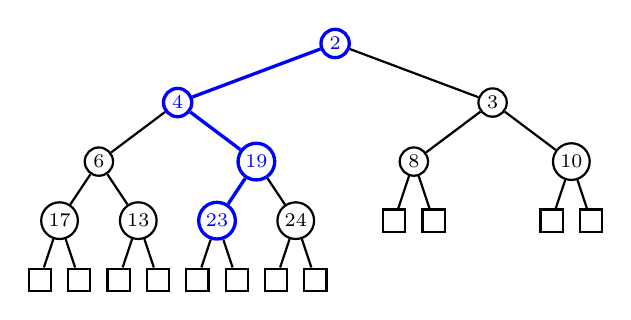
\begin{tikzpicture}
[-,thick,%
  every node/.style={shape=circle,inner sep=1.5pt,draw,thick},%
  scale=0.5]
\scriptsize
\node[blue,very thick] {$2$}
  [sibling distance=8cm]
  child[blue,very thick] {node[blue,very thick] {$4$}
    [sibling distance=4cm]
    child[black,thick] {node {$6$}
      [sibling distance=2cm]
      child {node {$17$}
        [sibling distance=1cm]
        child {node[rectangle,inner sep=4pt,draw,thick] {}}
        child {node[rectangle,inner sep=4pt,draw,thick] {}}
      }
      child {node {$13$}
        [sibling distance=1cm]
        child {node[rectangle,inner sep=4pt,draw,thick] {}}
        child {node[rectangle,inner sep=4pt,draw,thick] {}}
      }
    }
    child[blue,very thick] {node[blue,very thick] {$19$}
      [sibling distance=2cm]
      child[blue,very thick] {node[blue,very thick] {$23$}
        [sibling distance=1cm]
        child[black,thick] {node[rectangle,inner sep=4pt,draw,thick] {}}
        child[black,thick] {node[rectangle,inner sep=4pt,draw,thick] {}}
      }
      child[black,thick] {node {$24$}
        [sibling distance=1cm]
        child {node[rectangle,inner sep=4pt,draw,thick] {}}
        child {node[rectangle,inner sep=4pt,draw,thick] {}}
      }
    }
  }
  child {node {$3$}
    [sibling distance=4cm]
    child {node {$8$}
      [sibling distance=1cm]
      child {node[rectangle,inner sep=4pt,draw,thick] {}}
      child {node[rectangle,inner sep=4pt,draw,thick] {}}
    }
    child {node {$10$}
      [sibling distance=1cm]
      child {node[rectangle,inner sep=4pt,draw,thick] {}}
      child {node[rectangle,inner sep=4pt,draw,thick] {}}
    }
  };
\end{tikzpicture}
}

\caption{Delete and sift-down in a binary heap.}
\label{fig:tree_data_structures:delete_sift_down_binary_heap}
\end{figure}

\begin{algorithm}[!htbp]
%%%%%%%%%%%%%%%%%%%%%%%%%%%%%%%%%%%%%%%%%%%%%%%%%%%%%%%%%%%%%%%%%%%%%%%%%%%
%% This file is part of the book
%%
%% Algorithmic Graph Theory
%% http://code.google.com/p/graph-theory-algorithms-book/
%%
%% Copyright (C) 2009, 2010 Minh Van Nguyen <nguyenminh2@gmail.com>
%%
%% See the file COPYING for copying conditions.
%%%%%%%%%%%%%%%%%%%%%%%%%%%%%%%%%%%%%%%%%%%%%%%%%%%%%%%%%%%%%%%%%%%%%%%%%%%

\DontPrintSemicolon
\SetAlgoNoLine
%%
%% data section
\SetKwInOut{Input}{Input}
\SetKwInOut{Output}{Output}
\SetKwData{MyLeft}{left}
\SetKwData{MyRight}{right}
\SetKwData{MyRoot}{root}
\SetKwData{MyTrue}{true}
%%
%% input/output
\Input{A binary heap $T$, given in sequence representation, having
  $n > 1$ internal vertices.}
\Output{Extract the minimum vertex of $T$. With one vertex removed,
  $T$ must satisfy the heap-order property.}
\BlankLine
%%
%% algorithm body
$\MyRoot \assign T[0]$\;
$n \assign n - 1$\;
$v \assign T[n]$\;
$i \assign 0$\;
$j \assign 0$\;
\While{$\MyTrue$}{
  $\MyLeft \assign 2i + 1$\;
  $\MyRight \assign 2i + 2$\;
  \If{\rm $\MyLeft < n$ and $\kappa_{T[\MyLeft]} \leq \kappa_v$}{
    \eIf{\rm $\MyRight < n$ and $\kappa_{T[\MyRight]} \leq \kappa_{T[\MyLeft]}$}{
      $j \assign \MyRight$\;
    }{
      $j \assign \MyLeft$\;
    }
  }
  \ElseIf{\rm $\MyRight < n$ and $\kappa_{T[\MyRight]} \leq \kappa_v$}{
    $j \assign \MyRight$\;
  }
  \Else{
    $T[i] \assign v$\;
    exit the loop\;
  }
  $T[i] \assign T[j]$\;
  $i \assign j$\;
}
\Return $\MyRoot$\;

\caption{Extract the minimum vertex of a binary heap.}
\label{alg:tree_data_structures:binary_heap_delete}
\end{algorithm}


%%%%%%%%%%%%%%%%%%%%%%%%%%%%%%%%%%%%%%%%%%%%%%%%%%%%%%%%%%%%%%%%%%%%%%%%%%%

\subsection{Constructing a binary heap}

Given a collection of $n$ vertices $v_0, v_1, \dots, v_{n-1}$ with
corresponding keys $k_0, k_1, \dots, k_{n-1}$, we want to construct a
binary heap containing exactly those vertices. A basic approach is to
start with a trivial tree and build up a binary heap via successive
insertions. As each insertion requires $O(\lg n)$ time, the method of
binary heap construction via successive insertion of each of the $n$
vertices requires $O(n \cdot \lg n)$ time. It turns out we could do a
bit better and achieve the same result in linear time.

\begin{algorithm}[!htbp]
%%%%%%%%%%%%%%%%%%%%%%%%%%%%%%%%%%%%%%%%%%%%%%%%%%%%%%%%%%%%%%%%%%%%%%%%%%%
%% This file is part of the book
%%
%% Algorithmic Graph Theory
%% http://code.google.com/p/graph-theory-algorithms-book/
%%
%% Copyright (C) 2009, 2010, 2011 Minh Van Nguyen <nguyenminh2@gmail.com>
%%
%% See the file COPYING for copying conditions.
%%%%%%%%%%%%%%%%%%%%%%%%%%%%%%%%%%%%%%%%%%%%%%%%%%%%%%%%%%%%%%%%%%%%%%%%%%%

\DontPrintSemicolon
\SetAlgoNoLine
%%
%% data section
\SetKwInOut{Input}{Input}
\SetKwInOut{Output}{Output}
\SetKwData{MyLeft}{left}
\SetKwData{MyRight}{right}
\SetKwData{MyTrue}{true}
%%
%% input/output
\Input{A binary tree $T$, given in sequence representation, having
  $n > 1$ internal vertices.}
\Output{The binary tree $T$ heapified so that it satisfies the
  heap-order property.}
\BlankLine
%%
%% algorithm body
\For{$i \assign \lfloor n/2 \rfloor - 1, \dots, 0$}{
  $v \assign T[i]$\;
  $j \assign 0$\;
  \While{$\MyTrue$}{
    $\MyLeft \assign 2i + 1$\;
    $\MyRight \assign 2i + 2$\;
    \If{\rm $\MyLeft < n$ and $\kappa_{T[\MyLeft]} \leq \kappa_v$}{
      \eIf{\rm $\MyRight < n$ and $\kappa_{T[\MyRight]} \leq \kappa_{T[\MyLeft]}$}{
        $j \assign \MyRight$\;
      }{
        $j \assign \MyLeft$\;
      }
    }
    \ElseIf{\rm $\MyRight < n$ and $\kappa_{T[\MyRight]} \leq \kappa_v$}{
      $j \assign \MyRight$\;
    }
    \Else{
      $T[i] \assign v$\;
      exit the while loop\;
    }
    $T[i] \assign T[j]$\;
    $i \assign j$\;
  }
}
\Return $T$\;

\caption{Heapify a binary tree.}
\label{alg:tree_data_structures:heapify_binary_tree}
\end{algorithm}

A better approach starts by letting $v_0, v_1, \dots, v_{n-1}$ be the
internal vertices of a binary tree $T$. The tree $T$ need not satisfy
the heap-order property, but it must satisfy the heap-structure
property. Suppose $T$ is given in sequence representation so that we
have the correspondence $v_i = T[i]$ and the last internal vertex of
$T$ has index $n - 1$. The parent of $T[n-1]$ has index
\[
j
=
\left\lfloor \frac{n - 1}{2} \right\rfloor.
\]
Any vertex of $T$ with sequence index beyond $n - 1$ is a leaf. In
other words, if an internal vertex has index $> j$, then the children
of that vertex are leaves and have indices $\geq n$. Thus any internal
vertex with index $\geq \lfloor n/2 \rfloor$ has leaves for its
children. Conclude that internal vertices with indices
%%
\begin{equation}
\label{eqn:tree_data_structures:index_internal_vertices_with_leaves}
\left\lfloor \frac{n}{2} \right\rfloor,\,
\left\lfloor \frac{n}{2} \right\rfloor + 1,\,
\left\lfloor \frac{n}{2} \right\rfloor + 2,
\dots,
n - 1.
\end{equation}
%%
have only leaves for their children.

Our next task is to ensure that the heap-order property holds for
$T$. If $v$ is an internal vertex with index
in~\eqref{eqn:tree_data_structures:index_internal_vertices_with_leaves},
then the subtree rooted at $v$ is trivially a binary heap. Consider
the indices from $\lfloor n / 2 \rfloor - 1$ all the way down to
$0$ and let $i$ be such an index, i.e. let
$0 \leq i \leq \lfloor n / 2 \rfloor - 1$. We heapify the subtree of
$T$ rooted at $T[i]$, effectively performing a sift-down on this
subtree. Once we have heapified all subtrees rooted at $T[i]$ for
$0 \leq i \leq \lfloor n / 2 \rfloor - 1$, the resulting tree $T$ is a
binary heap. Our discussion is summarized in
Algorithm~\ref{alg:tree_data_structures:heapify_binary_tree}.

Earlier in this section, we claimed that
Algorithm~\ref{alg:tree_data_structures:heapify_binary_tree} can be
used to construct a binary heap in worst-case linear time. To prove
this, let $T$ be a binary tree satisfying the heap-structure property
and having $n$ internal vertices. By
Corollary~\ref{cor:tree_data_structures:height_binary_heap}, $T$ has
height $h = \lceil \lg(n + 1) \rceil$. We perform a sift-down for at
most $2^i$ vertices of depth $i$, where each sift-down for a subtree
rooted at a vertex of depth $i$ takes $O(h - i)$ time. Then the total
time for Algorithm~\ref{alg:tree_data_structures:heapify_binary_tree}
is
%%
\begin{align*}
O\left( \sum_{0 \leq i < h} 2^i (h - i) \right)
&=
O\left( 2^h \sum_{0 \leq i < h} \frac{2 - i} {2^{h - i}} \right) \\[4pt]
&=
O\left( 2^h \sum_{k > 0} \frac{k}{2^k} \right) \\[4pt]
&=
O\left( 2^{h + 1} \right) \\[4pt]
&=
O(n)
\end{align*}
%%
where we used the closed form $\sum_{k > 0} k / 2^k = 2$ for a
geometric series and
Theorem~\ref{thm:trees_forests:complete_binary_tree_exact_order}.


%%%%%%%%%%%%%%%%%%%%%%%%%%%%%%%%%%%%%%%%%%%%%%%%%%%%%%%%%%%%%%%%%%%%%%%%%%%

\section{Binomial heaps}
\index{binomial heap}

We are given two binary heaps $T_1$ and $T_2$ and we want to merge
them into a single heap. We could start by choosing to insert each
element of $T_2$ into $T_1$, successively extracting the minimum
element from $T_2$ and insert that minimum element into $T_1$. If
$T_1$ and $T_2$ have $m$ and $n$ elements, respectively, we would
perform $n$ extractions from $T_2$ totalling
\[
O\left( \sum_{0 < k \leq n} \lg k \right)
\]
time and inserting all of the extracted elements from $T_2$ into
$T_1$ requires a total runtime of
%%
\begin{equation}
\label{eqn:tree_data_structures:total_runtime_inserting_n_extra_elements}
O\left( \sum_{n \leq k < n + m} \lg k \right).
\end{equation}
%%
We approximate the addition of the two sums by
\[
\int_0^{n + m} \lg k \; dk
=
\left. \frac{k \cdot \ln k - k} {\ln 2} + C \right|_{k=0}^{k=n+m}
\]
for some constant $C$. The above method of successive extraction and
insertion therefore has a total runtime of
\[
O\left( \frac{(n + m) \cdot \ln(n + m) - n - m} {\ln 2} \right).
\]
for merging two binary heaps.

Alternatively, we could slightly improve the latter runtime for
merging $T_1$ and $T_2$ by successively extracting the last internal
vertex of $T_2$. The whole process of extracting all elements from
$T_2$ in this way takes $O(n)$ time and inserting each of the
extracted elements into $T_1$ still requires the runtime in
expression~\eqref{eqn:tree_data_structures:total_runtime_inserting_n_extra_elements}.
We approximate the sum
in~\eqref{eqn:tree_data_structures:total_runtime_inserting_n_extra_elements}
by
\[
\int_{k=n}^{k=n+m} \lg k \; dk
=
\left. \frac{k \cdot \ln k - k} {\ln 2} + C \right|_{k=n}^{k=n+m}
\]
for some constant $C$. Therefore, the improved extraction and
insertion method requires
\[
O\left(
\frac{(n+m) \cdot \ln(n+m) - n \cdot \ln n - m} {\ln 2} - n
\right)
\]
time in order to merge $T_1$ and $T_2$.

Can we improve on the latter runtime for merging two binary heaps? It
turns out we can by using a type of mergeable heap called
binomial\index{binomial heap} heap that supports merging two heaps in
logarithmic time.


%%%%%%%%%%%%%%%%%%%%%%%%%%%%%%%%%%%%%%%%%%%%%%%%%%%%%%%%%%%%%%%%%%%%%%%%%%%

\subsection{Binomial trees}
\index{binomial tree}

A binomial heap can be considered as a collection of binomial
trees. The binomial tree of order $k$ is denoted $B_k$ and defined
recursively as follows:
%%
\begin{enumerate}
\item The binomial tree of order $0$ is the trivial tree.

\item The binomial tree of order $k > 0$ is a rooted tree, where from
  left to right the children of the root of $B_k$ are roots of
  $B_{k-1}, B_{k-2}, \dots, B_0$.
\end{enumerate}
%%
Various examples of binomial trees are shown in
Figure~\ref{fig:tree_data_structures:binomial_trees_k0_4}. The
binomial tree $B_k$ can also be defined as follows. Let $T_1$ and
$T_2$ be two copies of $B_{k-1}$ with root vertices $r_1$ and $r_2$,
respectively. Then $B_k$ is obtained by letting, say, $r_1$ be the
left-most child of $r_2$.
Lemma~\ref{lem:tree_data_structures:basic_properties_binomial_trees}
lists various basic properties of binomial trees. Property~(3) of
Lemma~\ref{lem:tree_data_structures:basic_properties_binomial_trees}
uses the binomial\index{binomial coefficient} coefficient, from whence
$B_k$ derives its name.

\begin{figure}[!htbp]
\centering
%%%%%%%%%%%%%%%%%%%%%%%%%%%%%%%%%%%%%%%%%%%%%%%%%%%%%%%%%%%%%%%%%%%%%%%%%%%
%% This file is part of the book
%%
%% Algorithmic Graph Theory
%% http://code.google.com/p/graph-theory-algorithms-book/
%%
%% Copyright (C) 2009, 2010 Minh Van Nguyen <nguyenminh2@gmail.com>
%%
%% See the file COPYING for copying conditions.
%%%%%%%%%%%%%%%%%%%%%%%%%%%%%%%%%%%%%%%%%%%%%%%%%%%%%%%%%%%%%%%%%%%%%%%%%%%

\subfigure[$B_0$]{
\begin{tikzpicture}
[nodeDecorate/.style={shape=circle,inner sep=2pt,draw,thick}]
%% nodes or vertices
\node (1) at (0,0) [nodeDecorate] {};
%% stub nodes that should not be visible
\node () at (-0.5,0) [] {};
\node () at (0.5,0) [] {};
\end{tikzpicture}
}
%%
%%
\quad
\subfigure[$B_1$]{
\begin{tikzpicture}
[-,thick]
\node[shape=circle,inner sep=2pt,draw,thick] {}
  child {node[shape=circle,inner sep=2pt,draw,thick] {}};
%% stub nodes that should not be visible
\node () at (-0.5,0) [] {};
\node () at (0.5,0) [] {};
\end{tikzpicture}
}
%%
%%
\quad
\subfigure[$B_2$]{
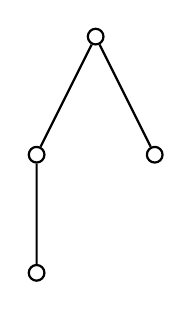
\begin{tikzpicture}
[-,thick,%
  every node/.style={shape=circle,inner sep=2pt,draw,thick}]
\node {}
  child {node {}
    child {node {}}
  }
  child {node {}};
\end{tikzpicture}
}
%%
%%
\quad
\subfigure[$B_3$]{
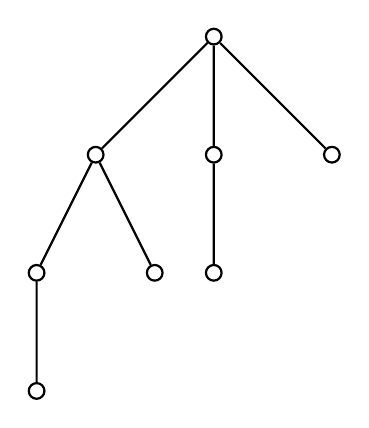
\begin{tikzpicture}
[-,thick,%
  every node/.style={shape=circle,inner sep=2pt,draw,thick}]
\node {}
  child {node {}
    child {node {}
      child {node {}}
    }
    child {node {}}
  }
  child {node {}
    child {node {}}
  }
  child {node {}};
\end{tikzpicture}
}
%%
%%
\subfigure[$B_4$]{
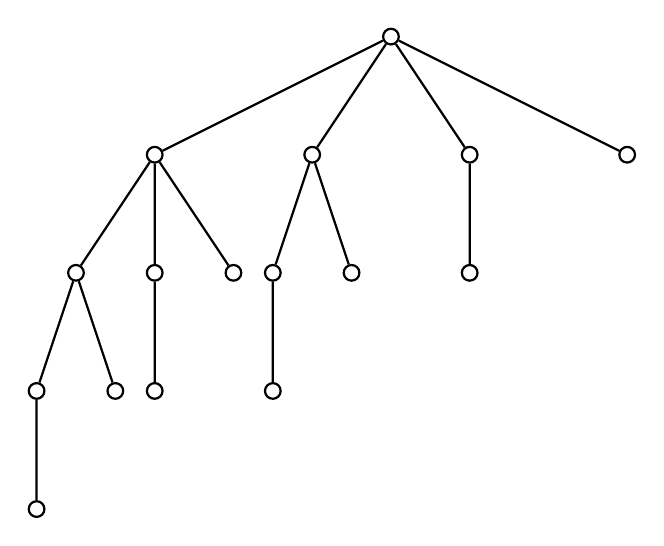
\begin{tikzpicture}
[-,thick,%
  every node/.style={shape=circle,inner sep=2pt,draw,thick}]
\node {}
  [sibling distance=2cm]
  child {node {}
    [sibling distance=1cm]
    child {node {}
      child {node {}
        child {node {}}
      }
      child {node {}}
    }
    child {node {}
      child {node {}}
    }
    child {node {}}
  }
  child {node {}
    [sibling distance=1cm]
    child {node {}
      child {node {}}
    }
    child {node {}}
  }
  child {node {}
    [sibling distance=1cm]
    child {node {}}
  }
  child {node {}};
\end{tikzpicture}
}

\caption{Binomial trees $B_k$ for $k = 0, 1, 2, 3, 4, 5$.}
\label{fig:tree_data_structures:binomial_trees_k0_4}
\end{figure}

\begin{lemma}
\label{lem:tree_data_structures:basic_properties_binomial_trees}
\textbf{Basic properties of binomial trees.}
Let $B_k$ be a binomial tree of order $k \geq 0$. Then the following
properties hold:
%%
\begin{enumerate}
\item The order of $B_k$ is $2^k$.

\item The height of $B_k$ is $k$.

\item For $0 \leq i \leq k$, we have $\binom{k}{i}$ vertices at depth
  $i$.

\item The root of $B_k$ is the only vertex with maximum degre
  $\Delta(B_k) = k$. If the children of the root are numbered
  $k - 1, k - 2, \dots, 0$ from left to right, then child $i$ is the
  root of the subtree $B_i$.
\end{enumerate}
\end{lemma}

\begin{proof}
We use induction on $k$. The base case for each of the above
properties is $B_0$, which trivially holds.

(1)~By our inductive hypothesis, $B_{k-1}$ has order $2^{k-1}$. Since
$B_k$ is comprised of two copies of $B_{k-1}$, conclude that $B_k$ has
order
\[
2^{k-1} + 2^{k-1}
=
2^k.
\]

(2)~The binomial tree $B_k$ is comprised of two copies of $B_{k-1}$,
the root of one copy being the left-most child of the root of the
other copy. Then the height of $B_k$ is one greater than the height of
$B_{k-1}$. By our inductive hypothesis, $B_{k-1}$ has height $k - 1$
and therefore $B_k$ has height $(k - 1) + 1 = k$.

(3)~Denote by $D(k,i)$ the number of vertices of depth $i$ in
$B_k$. As $B_k$ is comprised of two copies of $B_{k-1}$, a vertex at
depth $i$ in $B_{k-1}$ appears once in $B_k$ at depth $i$ and a second
time at depth $i + 1$. By our inductive hypothesis,
%%
\begin{align*}
D(k,i)
&=
D(k-1, i) + D(k-1, i-1) \\[4pt]
&=
\binom{k-1}{i} + \binom{k-1}{i-1} \\[4pt]
&=
\binom{k}{i}
\end{align*}
%%
where we used Pascal's\index{Pascal!formula} formula which states that
\[
\binom{n+1}{r}
=
\binom{n}{r-1} + \binom{n}{r}
\]
for any positive integers $n$ and $r$ with $r \leq n$.

(4)~This property follows from the defintion of $B_k$.
\end{proof}

\begin{corollary}
If a binomial tree has order $n \geq 0$, then the degree of any vertex
$i$ is bounded by $\deg(i) \leq \lg n$.
\end{corollary}

\begin{proof}
Apply properties~(1) and~(4) of
Lemma~\ref{lem:tree_data_structures:basic_properties_binomial_trees}.
\end{proof}


%%%%%%%%%%%%%%%%%%%%%%%%%%%%%%%%%%%%%%%%%%%%%%%%%%%%%%%%%%%%%%%%%%%%%%%%%%%

\subsection{Binomial heaps}
\index{binomial heap}

A binomial\index{binomial heap} heap $H$ can be considered as a
collection of binomial trees. Each vertex in $H$ has a corresponding
key and all vertex keys of $H$ belong to a totally ordered set having
total order $\leq$. The heap also satisfies the following
\emph{binomial heap properties}\index{binomial heap!properties}:
%%
\begin{description}
\item[Heap-order property:]\index{heap-order property}
  Let $B_k$ be a binomial tree in $H$. If $v$ is a vertex of $B_k$
  other than the root and $p$ is the parent of $v$ and having
  corresponding keys $k_v$ and $k_p$, respectively, then
  $k_p \leq k_v$.

\item[Root-degree property:]\index{root-degree property}
  For any integer $k \geq 0$, $H$ contains at most one binomial tree
  whose root has degree $k$.
\end{description}


%%%%%%%%%%%%%%%%%%%%%%%%%%%%%%%%%%%%%%%%%%%%%%%%%%%%%%%%%%%%%%%%%%%%%%%%%%%

\section{Binary search trees}

See section~3.6 of Gross and Yellen~\cite{GrossYellen1999}, and
chapter~12 of Cormen~et~al.~\cite{CormenEtAl2001}. See also
\url{http://en.wikipedia.org/wiki/Binary_search_tree}.


\begin{itemize}
\item records and keys

\item searching a binary search tree (BST)

\item inserting into a BST

\item deleting from a BST

\item traversing a BST

\item sorting using BST
\end{itemize}

A {\it binary search tree} (BST) is a rooted binary tree
$T=(V,E)$ having weighted vertices ${\rm wt}:V\to \R$ satisfying:
\index{binary search tree}
\index{BST}

\begin{itemize}
\item
 The left subtree of a vertex $v$ contains only vertices whose label
(or ``key'') is less than the label of $v$.
\item
The right subtree of a vertex $v$ contains only vertices whose label
  is greater than the label of $v$.
\item
Both the left and right subtrees must also be binary search trees.
\end{itemize}

From the above properties it naturally follows that:
{\it Each vertex has a distinct label.}


\subsubsection{Traversal}

The vertices of a BST $T$ can be visited retrieved in-order of the
weights of the vertices (i.e.,
using a symmetric search type) by recursively  traversing the left subtree of the
root vertex, then accessing the root vertex itself, then recursively traversing the
right subtree of the root node.

\subsubsection{Searching}

We are given a BST (i.e., a binary rooted tree with weighted vertices
having distinct weights satisfying the above criteria) $T$ and a
label $\ell$. For this search, we are looking for a vertex in $T$
whose label is $\ell$, if one exists.

We begin by examining the root vertex, $v_0$. If $\ell={\rm wt}(v_0)$,
the search is successful. If the $\ell<{\rm wt}(v_0)$,
search the left subtree. Similarly, if $\ell>{\rm wt}(v_0)$,
search the right subtree. This process is repeated until a vertex
$v\in V$ is found for which $\ell={\rm wt}(v)$,
or the indicated subtree is empty.


\subsubsection{Insertion}

We are given a BST (i.e., a binary rooted tree with weighted vertices
having distinct weights satisfying the above criteria) $T$ and a
label $\ell$. We assume $\ell$ is between the
lowest weight of $T$ and the highest weight.
For this procedure, we are looking for a ``parent''
vertex in $T$ which can ``adopt'' a new vertex $v$ having weight $\ell$
and for which this augmented tree $T\cup v$ satisfies
the criteria above.

Insertion proceeds as a search does. However, in this case, you are
searching for vertices $v_1,v_2\in V$ for which
${\rm wt}(v_1)<\ell < {\rm wt}(v_2)$. Once found, these
vertices will tell you where to insert $v$.

\subsubsection{Deletion}

As above, we are given a BST $T$ and a
label $\ell$. We assume $\ell$ is between the
lowest weight of $T$ and the highest weight.
For this procedure, we are looking for a vertex $v$ of
$T$ which has weight $\ell$. We want to remove $v$ from
$T$ (and therefore also the weight $\ell$ from the list of weights),
thereby creating a ``smaller'' tree $T- v$ satisfying
the criteria above.

Deletion proceeds as a search does. However, in this case, you are
searching for vertex $v\in V$ for which
${\rm wt}(v)=\ell$. Once found, we remove $v$ from $V$
and any edge $(u,v)\in E$ is replaced by $(u,w_1)$
and $(u,w_2)$, where $w_1.w_2\in V$ were the children of $v$
in $T$.

\subsubsection{Sorting}

A binary search tree can be used to implement a simple but efficient
sorting algorithm. Suppose we wish to sort a list of numbers
$L = [\ell_1, \ell_2,\dots, \ell_n]$. First, let $V=\{1,2,\dots,n\}$
be the vertices of a tree and weight vertex $i$ with $\ell_i$,
for $1\leq i\leq n$. In this case, we can traverse this tree
in order of its weights, thereby building a BST recursively.
This BST represents the sorting of the list $L$.
Generally, the information represented by each vertex is a
record (or list or dictionary), rather than a single data element. However,
for sequencing purposes, vertices are compared according to their
labels rather than any part of their associated records.

\subsubsection{Traversal}

The vertices of a BST $T$ can be visited retrieved in-order of the
weights of the vertices (i.e.,
using a symmetric search type) by recursively  traversing the left subtree of the
root vertex, then accessing the root vertex itself, then recursively traversing the
right subtree of the root node.

\subsubsection{Searching}

We are given a BST (i.e., a binary rooted tree with weighted vertices
having distinct weights satisfying the above criteria) $T$ and a
label $\ell$. For this search, we are looking for a vertex in $T$
whose label is $\ell$, if one exists.

We begin by examining the root vertex, $v_0$. If $\ell={\rm wt}(v_0)$,
the search is successful. If the $\ell<{\rm wt}(v_0)$,
search the left subtree. Similarly, if $\ell>{\rm wt}(v_0)$,
search the right subtree. This process is repeated until a vertex
$v\in V$ is found for which $\ell={\rm wt}(v)$,
or the indicated subtree is empty.


\subsubsection{Insertion}

We are given a BST (i.e., a binary rooted tree with weighted vertices
having distinct weights satisfying the above criteria) $T$ and a
label $\ell$. We assume $\ell$ is between the
lowest weight of $T$ and the highest weight.
For this procedure, we are looking for a ``parent''
vertex in $T$ which can ``adopt'' a new vertex $v$ having weight $\ell$
and for which this augmented tree $T\cup v$ satisfies
the criteria above.

Insertion proceeds as a search does. However, in this case, you are
searching for vertices $v_1,v_2\in V$ for which
${\rm wt}(v_1)<\ell < {\rm wt}(v_2)$. Once found, these
vertices will tell you where to insert $v$.

\subsubsection{Deletion}

As above, we are given a BST $T$ and a
label $\ell$. We assume $\ell$ is between the
lowest weight of $T$ and the highest weight.
For this procedure, we are looking for a vertex $v$ of
$T$ which has weight $\ell$. We want to remove $v$ from
$T$ (and therefore also the weight $\ell$ from the list of weights),
thereby creating a ``smaller'' tree $T- v$ satisfying
the criteria above.

Deletion proceeds as a search does. However, in this case, you are
searching for vertex $v\in V$ for which
${\rm wt}(v)=\ell$. Once found, we remove $v$ from $V$
and any edge $(u,v)\in E$ is replaced by $(u,w_1)$
and $(u,w_2)$, where $w_1.w_2\in V$ were the children of $v$
in $T$.

\subsubsection{Sorting}

A binary search tree can be used to implement a simple but efficient
sorting algorithm. Suppose we wish to sort a list of numbers
$L = [\ell_1, \ell_2,\dots, \ell_n]$. First, let $V=\{1,2,\dots,n\}$
be the vertices of a tree and weight vertex $i$ with $\ell_i$,
for $1\leq i\leq n$. In this case, we can traverse this tree
in order of its weights, thereby building a BST recursively.
This BST represents the sorting of the list $L$.


%%%%%%%%%%%%%%%%%%%%%%%%%%%%%%%%%%%%%%%%%%%%%%%%%%%%%%%%%%%%%%%%%%%%%%%%%%%

\section{Problems}

\begin{problem}
\item Let $Q$ be a priority queue of $n > 1$ elements, given in
  sequence representation. From
  section~\ref{subsec:tree_data_structures:sequence_implementation},
  we know that inserting an element into $Q$ takes $O(n)$ time and
  deleting an element from $Q$ takes $O(1)$ time.
  %%
  \begin{enumerate}[(a)]
  \item Suppose $Q$ is an empty priority queue and let
    $e_0, e_1, \dots, e_n$ be $n + 1$ elements we want to insert into
    $Q$. What is the total runtime required to insert all the $e_i$
    into $Q$ while also ensuring that the resulting queue is a
    priority queue?

  \item Let $Q = [e_0, e_1, \dots, e_n]$ be a priority queue of
    $n + 1$ elements. What is the total time required to remove all
    the elements of $Q$?
  \end{enumerate}

\item Prove the correctness of
  Algorithms~\ref{alg:tree_data_structures:binary_heap_insert}
  and~\ref{alg:tree_data_structures:binary_heap_delete}.

\item Describe a variant of
  Algorithm~\ref{alg:tree_data_structures:binary_heap_delete} for
  modifying the key of the root of a binary heap, without extracting
  any vertex from the heap.

\item Section~\ref{subsec:tree_data_structures:insertion_sift_up}
  describes how to insert an element into a binary heap $T$. The
  general strategy is to choose the first leaf following the last
  internal vertex of $T$, replace that leaf with the new element so
  that it becomes an internal vertex, and perform a sift-up operation
  from there. If instead we choose any leaf of $T$ and replace that
  leaf with the new element, explain why we cannot do any better than
  Algorithm~\ref{alg:tree_data_structures:binary_heap_insert}.

\item Section~\ref{subsec:tree_data_structures:deletion_sift_down}
  shows how to extract the minimum vertex from a binary heap
  $T$. Instead of replacing the root with the last internal vertex of
  $T$, we could replace the root with any other vertex of $T$ that is
  not a leaf and then proceed to maintain the heap-structure and
  heap-order properties. Explain why the latter strategy is not better
  than Algorithm~\ref{alg:tree_data_structures:binary_heap_delete}.

\item Let $S$ be a sequence of $n > 1$ real numbers. How can we use
  algorithms described in
  section~\ref{sec:tree_data_structures:binary_heaps} to sort $S$?

\item The binary heaps discussed in
  section~\ref{sec:tree_data_structures:binary_heaps} are properly
  called minimum\index{binary heap!minimum} binary heaps because the
  root of the heap is always the minimum vertex. A corresponding
  notion is that of maximum\index{binary heap!maximum} binary heaps,
  where the root is always the maximum element. Describe algorithms
  analogous to those in
  section~\ref{sec:tree_data_structures:binary_heaps} for managing
  maximum binary heaps.
\end{problem}
